\section{Scientific motivation}\label{scientific-motivation}

An inverse image can look geologically persuasive even when multiple
models explain the data, the assumed physics are violated, or a withheld
acquisition subset is poorly predicted. This is familiar across
geophysics: potential-field inverses are non-unique; MT dimensionality
and component quality condition whether a 1D interpretation is
defensible; seismic inversion depends on illumination, bandwidth,
starting model, and cycle skipping; and coupled or learned estimates
inherit their structural or training priors. A low objective is evidence
about a specified objective under a specified data model. By itself, it
is not evidence of unique or accurate geology.

The topic sequence draws on the public theoretical-practical geophysical
inversion course by Mantilla. Its notebooks, recordings, images, and raw
data are not redistributed. The source commit was
\texttt{0084021fcc6c1d2f112b144e6e5f0a3d92f20dff} (Mantilla course). The
research survey distinguishes primary sources from implementation
choices and identifies where the methods differ from cited work
(\url{docs/research/review.md}). The aim is to connect domain
assumptions, executable calculations, diagnostic evidence, and failure
states within one inspectable project.

The report covers gravity station correction and prism inversion,
aeromagnetic processing, induced-magnetization modelling,
magnetotelluric screening and layered-earth inversion, electrical
resistivity inversion, response-aware waveform processing, first-arrival
tomography, acoustic full-waveform inversion, joint potential-field
inversion, learned seismic-velocity estimation, and earthquake phase
picking. It also evaluates a proposed coverage-conditioned null-space
correction. Method definitions and numerical assumptions are in
\url{docs/design/SDD.md}.

\section{Software and evidence
design}\label{software-and-evidence-design}

\subsubsection{2.1 Evidence chain}\label{evidence-chain}

The intended data flow follows the path

\texttt{source\ →\ immutable\ raw\ asset\ →\ validated\ dataset\ →\ processing\ →\ model/survey\ →\ solve\ →\ evaluation\ →\ result/export}.

At each boundary the contracts carry modality, named dimensions and
order, coordinate frame or specified local coordinates, units, geometry,
masks and reasons, uncertainty, parent identities, code/environment
information, and hashes as applicable. Unknown units, datum, signs,
component orientation, rights, or response conventions are reasons to
reject or quarantine an input rather than infer missing facts. Known
truth is attached only to explicitly synthetic cases. Field observations
may be screened and processed, but a synthetic constructor is never
substituted for missing field provenance or truth.

The application separates three execution contexts. Visitors can inspect
public material and use only those browser calculations whose
client-side behavior has been validated. Authenticated project workflows
are designed to isolate upload, ownership, and bounded worker execution
on the single canonical ML VPS origin. Larger training, extensive FWI,
and full bake workflows remain local CPU/GPU pipelines. A static or
browser replay of a saved artifact is not represented as an online
inverse solve. The specified deployment uses one bounded ML VPS service.
Its capacity and numerical job behavior have not been measured on the
live host.

\subsubsection{2.2 Reproducible software
artifacts}\label{reproducible-software-artifacts}

The software contains a Python data pipeline and solver implementations,
generated and source-controlled scientific outputs, JSON contracts and
validation outputs, frontend TypeScript/React instruments, and
computational notebooks in English and Spanish. The user-facing browser
is intended to display computed arrays and explicit physical axes, not
to invent a second approximate result for animation. Physical result
records distinguish observations, predictions, signed residuals, model
values, objective terms, coverage and uncertainty diagnostics, stopping
state, and provenance. Display interpolation or color mapping is a
rendering operation and must not be mistaken for increased model
resolution.

Notebooks are part of the research material, not merely screenshots.
Their lessons explain assumptions, execute the named calculations, show
numerical outputs, compare with independent identities or baselines when
available, and retain unresolved results. The bilingual content was
corrected where translations, counts, or numerical interpretations
differed. Execution and translation checks establish neither field
validity nor educational efficacy.

\section{Data and experimental scope}\label{data-and-experimental-scope}

\subsubsection{3.1 Authored synthetic
experiments}\label{authored-synthetic-experiments}

The original canonical suite uses independently constructed geological
geometries instead of repeating one centered anomaly. Its earlier 0.04
report describes 20 distinct cases and six controlled conditions per
case (120 experiments, 348 method results). The conditions vary
contrast, noise, acquisition, coverage, or regularization according to
the physical family; they are not interchangeable perturbations and are
not samples from a geological population. Later repository work adds
separate survey, uploaded-data, learning, and source-screening
experiments. Therefore the older 120-experiment suite is a defined
artifact family, not a count of every experiment now present in the
repository.

Synthetic constructors provide known truth for controlled tests of
forward physics and conditional inversion behavior. They do not encode
the full complexity of field geology. Noise perturbations at fixed
mesh/prior/tradeoff measure conditional estimator repeatability, not
posterior uncertainty. A held-out line, shot, family, or acquisition
tests only the specified split and comparator. Repeated numerical trials
from one generator do not establish field performance.

\subsubsection{3.2 External data and
eligibility}\label{external-data-and-eligibility}

Two SimPEG tutorial archives are independently pinned and locally
preprocessed as ingestion examples. The source documentation states that
their derived observation tables are not redistributed while upstream
redistribution rights remain unresolved. They are not field validation.
The measured Clear Lake EDI station cl061 is hash-pinned and cited to
the USGS and EarthScope data releases
\cite{usgsClearLake,earthscopeClearLake}. Its impedance tensor fails the
required 1D consistency screen; it remains a QC-only dataset, and no
layered inversion or geological result is claimed.

Other data paths include provider-linked or rights-restricted data. For
example, the Slagdump ERT raw asset is absent locally under its
provider-link-only status; focused notebook checks consequently skip
tests that require those bytes. The Koenigsee travel-time lesson is an
authored synthetic method control and does not establish execution on
the provider-linked case. The M13 STEAD excerpts \cite{mousavi2019} and
associated project-trained checkpoint have a scoped redistribution
decision with attribution; that decision does not generalize to other
data or establish model accuracy. Rights, data custody, field
eligibility, numerical correctness, and scientific validation remain
separate decisions.

\section{Methods}\label{methods}

The method identifiers below follow \url{docs/design/SDD.md}. Each entry
names an implementation and its tests; this does not imply validated use
for every input or a complete end-to-end workflow.

\begin{center}\small
\begin{longtable}{@{}>{\raggedright\arraybackslash}p{0.18\textwidth}>{\raggedright\arraybackslash}p{0.38\textwidth}>{\raggedright\arraybackslash}p{0.38\textwidth}@{}}
\toprule
Method & Executable purpose & Principal limitations \\
\midrule
\endfirsthead
\toprule
Method & Executable purpose & Principal limitations \\
\midrule
\endhead
Gravity corrections and transforms & Gravity station corrections, datum and uncertainty lineage, and transforms with safeguards against duplicate corrections. & Field eligibility still depends on exact source, datum, instrument, and uncertainty lineage. A local adapter pass does not validate arbitrary field tables. \\
Weighted 3D gravity prism inversion & Weighted 3D gravity prism forward/inverse calculations, including a bounded L2 survey inversion and comparison with independent prism physics. & Non-uniqueness persists; a good data fit or a visually compact body does not identify geology. Full-survey and field performance remain untested. \\
Aeromagnetic processing and continuation & Aeromagnetic line/tie-line/height checks, blocked line holdout, support-aware gridding, and physically supported upward continuation. & Authored survey controls do not establish broad provider-data validation or field magnetic inversion. \\
Induced-magnetization prism modelling & Induced-magnetization prism forward modelling and physical objective/derivative construction, checked against Choclo. & A full nonzero survey inverse with held-out evaluation is not included in the available evidence. Remanence violates the induced-direction assumption. \\
EDI quality and dimensionality screening & MT EDI component, variance, rotation, tipper, and dimensionality screening. & A tensor record is not automatically eligible for a 1D inverse. cl061 remains QC-only. \\
Layered-earth impedance inversion & Layered-earth complex-impedance response and bounded 1D inversion, with cross-checks against MTpy and browser/local analytic cases. & Known layer thickness and isotropic 1D assumptions constrain the synthetic inverse. The cl061 field screen fails. \\
Two-dimensional electrical resistivity inversion & 2D ERT processing/inversion with electrode geometry, topography, reciprocal/QC logic, blocked holdout, and explicit failed-inverse states. & Rights-restricted raw data are not fabricated or represented as executed; independent comparison and some field paths remain open. \\
Response-aware waveform processing & MiniSEED/StationXML waveform handling, response-aware filtering, STA/LTA or matched-arrival picks. & Response epochs, units, gaps, and channel orientation are strict eligibility conditions. STA/LTA picks are not universal truth labels. \\
First-arrival travel-time inversion & First-arrival travel-time inversion with explicit source/receiver geometry, bounded velocity, ray coverage, and held-out-shot comparison against a baseline. & The executed teaching control is synthetic and uses a straight-ray/Dijkstra model; the synthetic control does not represent provider-linked field data. \\
Acoustic full-waveform inversion & Acoustic constant-density FWI with Deepwave, bounded velocity updates, full-band and frequency-continuation schedules, active/withheld receiver diagnostics, and saved optimizer states. & Non-convexity, cycle skipping, limited illumination, inverse crime from using the same forward engine, and acoustic-only physics remain material limitations. Some cases improve model RMSE but fail the specified noise-consistency criterion. \\
Joint potential-field inversion & Joint potential-field inversion comparing uncoupled fits, spatial cross-gradient coupling, and an explicit Gaussian-mixture petrophysical prior. & The project Gaussian-mixture-prior implementation is not the SimPEG PGI optimizer. Coupling can trade one property against another; one calibration matrix does not establish general performance. \\
Learned seismic-velocity estimation & A learned seismic-velocity inversion trained on disjoint procedural families and compared with a same-input weighted L2 solve and independent quadrature forward operator. & The frozen joint family/acquisition holdout fails both prespecified ratios; training success does not override the held-out result. \\
PhaseNet-family phase picking & PhaseNet-family P/S inference \cite{zhu2019}, matched STA/LTA comparison, and local browser ONNX inference with explicit preprocessing and abstention rules. & Curated browser parity is runtime consistency, not accuracy. Population metrics come from the separate locked test cohort and analyst references, not geological truth. \\
Geometry-normalized travel-time residual refinement & Backprojected travel-time residuals are normalized by ray length and cell coverage, then supplied with the coverage field to a bounded residual CNN. & The current physics-v2 study fails both predeclared joint-shift ratios in the primary and same-seed replay. This is a negative synthetic comparison; null-space projection is established prior methodology and no superiority claim is made. \\
\bottomrule
\end{longtable}
\end{center}

\subsection{Method-specific mathematical formulations}
\label{method-formulations}

\subsubsection{Gravity station corrections and uncertainty}
\label{method-gravity-corrections}

The station workflow treats a gravity value as a measurement with a
history, not as an unlabeled scalar. Each row retains the source value,
station identifier, coordinate reference, elevation convention, unit,
instrument or provider correction state, and uncertainty. A correction
is applied only when the source record and selected operation establish
that it has not already been applied. Unknown metadata are preserved as
unknown and cause the corresponding derived quantity to be withheld;
the code does not infer a datum or silently convert a likely unit.
This fail-closed rule matters because a numerically plausible anomaly
can be produced from an incorrect sign, a duplicated free-air term, a
mixed reference datum, or a coordinate error.

For a station record $i$, the processed anomaly can be represented as
the source observation plus a vector of signed corrections and a
reference shift,
\begin{equation}
  g_i^{\mathrm{proc}} = g_i^{\mathrm{src}} + \mathbf{c}_i^{\mathsf T}\mathbf{a}
  + \Delta g_{\mathrm{datum}},
  \label{eq:gravity-corrections}
\end{equation}
where $\mathbf{c}_i$ contains only corrections supported by the
declared input and $\mathbf{a}$ contains their sign convention. This
notation is an accounting identity, not an assertion that every source
provides every correction. A missing correction value is not equivalent
to zero. The implementation keeps the source and derived columns
separate so a correction chain can be reproduced and audited. The
no-double-correction validator rejects a record whose declared state is
inconsistent with the requested chain before the output is emitted.

If source and correction errors are independent, the propagated
variance is the sum of their contributions. More generally, the
declared covariance is transformed by the same linear operation,
\begin{equation}
  \sigma_{i,\mathrm{proc}}^2 = \mathbf{a}_i^{\mathsf T}\,\mathbf{C}_i\,\mathbf{a}_i,
  \qquad
  \mathbf{C}_{\mathrm{proc}} = \mathbf{A}\,\mathbf{C}_{\mathrm{src}}\,\mathbf{A}^{\mathsf T}.
  \label{eq:gravity-uncertainty}
\end{equation}
Here $\mathbf{a}_i$ is the local coefficient vector for the scalar
record, whereas $\mathbf{A}$ is the complete linear map over a stacked
survey. A diagonal-only uncertainty output is justified only when the
input specifies independent errors or when the transform preserves
that assumption. The processor does not manufacture cross-station
covariance from marginal standard deviations.

Implementation is split between source parsing, unit and datum checks,
correction-state validation, deterministic calculation, and a result
receipt. The receipt binds each output to its parent asset and records
the applied correction sequence, uncertainty provenance, and the
implementation identity. The station tests exercise a known correction
lineage, unit conversion, reference handling, uncertainty propagation,
and rejection of duplicated or unknown operations. These tests prove
the declared cases and code paths; they do not establish that an
arbitrary downloaded table is a complete or eligible gravity survey.

The lesson is deliberately connected to the potential-field inverse
that follows. A station table can pass syntax checks while remaining
scientifically inadmissible because of an undocumented tide convention,
unresolved datum, missing terrain model, or provider-level correction
that cannot be reconstructed. The interface therefore separates raw
records from processed records and exposes the provenance of each
column. A user must be able to determine which values came from the
provider, which were calculated locally, and which remain unavailable.
No corrected anomaly is presented as subsurface density, and no
correction step is described as an inversion. The relevant executable
entry point is \url{data-pipeline/gravity_processing.py}; the stable
station contract and rejection tests are in
\url{tests/numerics/test_gravity_processing.py}.

The correction receipt also provides a practical way to compare
processing paths without conflating them with a subsurface model. A
reviewer can start from the same immutable station rows, select the
permitted correction flags, and compare each derived column and
uncertainty against a direct hand calculation. This check matters when
adapting provider tables: field names alone do not reveal whether a
Bouguer or terrain term is already included. The parser keeps the
original numeric value and source metadata so the anomaly can be
regenerated without overwriting the received record.

Coordinate conversion is handled as its own provenance step. It
preserves the source coordinate reference and transforms station
locations before any spatial derivative, gridding or prism sensitivity
is evaluated. The transformed coordinates, selected local origin and
axis order travel with the derived survey. A correction is never
reconstructed from display coordinates rounded for a map. That rounding
may be visually harmless and still unacceptable for a derivative or a
high-gradient terrain model. The result contract therefore separates
display formatting from the coordinates used in the forward
calculation.

\subsubsection{Weighted three-dimensional gravity prism inversion}

The objective and depth weighting are grounded in established minimum-structure inversions for gravity and magnetics \cite{liGrav1998,liMag1996}. The present mesh, data weights and calibration are product-specific and are not a reproduction of those published implementations.
\label{method-gravity-inversion}

The gravity inverse maps a discretized density contrast to observations
through a forward operator assembled from three-dimensional prism
responses. Let $\mathbf{m}$ contain cell density contrasts and let
$\mathbf{G}$ map those contrasts to vertical gravity at the observation
locations. For the declared linear density model, the prediction is
\begin{equation}
  \mathbf{d}_{\mathrm{pred}} = \mathbf{G}\mathbf{m},
  \qquad
  \mathbf{r}=\mathbf{d}_{\mathrm{obs}}-\mathbf{G}\mathbf{m}.
  \label{eq:gravity-prism-forward}
\end{equation}
The units of $\mathbf{m}$, geometry, coordinates and $\mathbf{d}$ are
checked at the interface. The mesh order is part of the numerical
contract; a vector reshaped in a different cell order may look smooth
but represents different physical cells.

The bounded L2 reference minimizes a noise-weighted data term together
with a model-space penalty,
\begin{equation}
  \Phi(\mathbf{m}) = \tfrac12\|\mathbf{W}_d(\mathbf{G}\mathbf{m}-\mathbf{d}_{\mathrm{obs}})\|_2^2
  + \tfrac{\beta}{2}\|\mathbf{W}_m(\mathbf{m}-\mathbf{m}_{\mathrm{ref}})\|_2^2,
  \qquad \mathbf{m}_{\min}\leq\mathbf{m}\leq\mathbf{m}_{\max}.
  \label{eq:gravity-l2-objective}
\end{equation}
The reference model, bounds, weighting, regularization, mesh, active
cells, and stopping conditions are reported as parameters of a run.
Weights may encode stated standard deviations, but they do not
transform a deterministic synthetic perturbation into a probability
model. The minimizer is conditional on the mesh, reference and penalty.
The reported model is not a unique geological image.

For a linear forward model the gradient and normal equations provide
an independently checkable oracle,
\begin{equation}
  \nabla\Phi(\mathbf{m}) = \mathbf{G}^{\mathsf T}\mathbf{W}_d^{\mathsf T}\mathbf{W}_d
  (\mathbf{G}\mathbf{m}-\mathbf{d}_{\mathrm{obs}})
  +\beta\mathbf{W}_m^{\mathsf T}\mathbf{W}_m(\mathbf{m}-\mathbf{m}_{\mathrm{ref}}).
  \label{eq:gravity-gradient}
\end{equation}
The project checks selected forward values against an independent prism
calculation, then compares the SimPEG-backed solve with a bounded
least-squares reference on the same data, survey, mesh and error model.
This separates a forward-kernel error from optimizer configuration
and from differences caused by changing the data or discretization.

Evaluation reports fitted and held-out predictions, weighted residual
statistics, sensitivity or coverage diagnostics, and model-recovery
metrics only when synthetic truth exists. The reference case
demonstrates why these quantities are not interchangeable: a weighted
WRMS near one coexists with a model correlation of 0.283 and a recovered
centroid near 570 m for a truth near 282 m. The datum fit is consistent
with the chosen scale, while the density distribution is unresolved.
Potential-field depth/volume tradeoffs and mesh dependence remain; a
single model slice cannot remove them. The implementation is
\url{data-pipeline/gravity_l2.py} and the bounded calibration is covered
by \url{tests/numerics/test_gravity_l2.py} and
\url{tests/numerics/test_gravity_l2_selection.py}. The full family of
solver outcomes, including ineligible or unresolved records, must be
retained in the result catalogue rather than reduced to its best-looking
case.

The choice of data weighting and regularization has measurable
consequences. Multiplying every data standard deviation by a common
factor changes the relative balance between fit and model penalty unless
$\beta$ is changed consistently. A comparison between two solvers is
controlled only when observations, covariance, active cells, reference,
bounds, regularization and stopping rules are shared. The locked L2
control matrix varies its declared case factors while keeping that
comparison contract explicit. It records solver status separately
from scientific recovery: termination proves that a numerical stopping
rule was reached, whereas recovery requires an independent truth metric
and can still fail.

The sensitivity matrix also explains why fit alone is insufficient for
claiming resolution. Columns of $\mathbf{G}$ with similar predictions
are difficult to distinguish in the measured geometry; the penalty
selects one member from a family of acceptable models. A cellwise
display should be read alongside data residuals, model regularization,
depth sensitivity and synthetic truth when it exists. Potential-field
depth/volume tradeoffs and mesh dependence remain. The browser may
interpolate colors for display but must not regrid the model into
apparent new resolution. This separation of mesh values from rendering
coordinates is necessary for physical interpretation.

The reference model and active-cell mask are part of the mathematical
problem, not cosmetic defaults. A different reference shifts the
regularization center; a different mesh changes the columns and
correlations of the sensitivity matrix; and a different standard
deviation changes the relative contribution of each observation.
Accordingly, the result record must preserve these values with the data
identity and solver configuration. The independent prism calculation
tests the forward sign and scale for its stated rectangular geometry,
while the inverse comparison evaluates a separate question: whether the
selected bounded, regularized model predicts the observed survey and
recovers the known synthetic target. Neither calculation transfers to
an arbitrary field survey without coordinate, datum, error, and source
eligibility review. The L2 solution is therefore reported as a
conditional estimate under a fully specified objective, not as the
uniquely determined density distribution.

\subsubsection{Aeromagnetic processing and harmonic continuation}
\label{method-aeromagnetic-processing}

The aeromagnetic workflow begins with flight-line geometry and provider
leveling provenance. It checks coordinates, line identifiers, sample
spacing, flight height, tie-line support, duplicate points, and data
gaps before interpolation. A blocked flight line is reserved for
evaluation before gridding; the withheld observations are not used to
choose a grid or tune its smoothing. This test is intentionally
different from randomly withholding nearby points, since spatially
adjacent samples can share the same acquisition error and geological
signal.

Potential fields in a source-free half-space satisfy Laplace's equation.
For a horizontal Fourier component with wavenumber magnitude $k$,
upward continuation by height $h$ applies the transfer function
\begin{equation}
  \widehat{T}(k_x,k_y,h) = \widehat{T}(k_x,k_y,0)\exp(-h\sqrt{k_x^2+k_y^2}).
  \label{eq:magnetic-continuation}
\end{equation}
Thus higher wavenumbers decay faster. The operation suppresses short
wavelength content and is not an inverse continuation: recovering the
surface field from an elevated grid would amplify noise. The implementation
validates the transfer against a single analytic harmonic with known
wavenumber and continuation height; the test is a physical identity,
not an assertion that a gridded field uniquely determines its sources.

Interpolation and support are represented separately. Let $\mathcal{S}$
be the sampled footprint and $\mathcal{D}$ the output grid. A prediction
outside an accepted support neighborhood is stored as unavailable,
not silently filled with a value that looks measured. The gridding
receipt records the interpolation rule, node spacing, coordinate frame,
input line selections, mask, and any height transform. This permits a
reviewer to distinguish the actual flight path from the raster display.
The interface displays both the raster and the original lines, along
with the blocked-line residuals and support mask.

The current public USGS Amargosa example uses the provider-levelled
channel without repeating upstream diurnal, IGRF, navigation, or
flight/tie-line levelling corrections. Its rights and source hash are
recorded in the research evidence; the calculation is a bounded
processing/QC example, not independent site validation or a magnetic
inversion. Upstream corrections cannot be reconstructed from absent
instrument and processing records. A different provider dataset would
need its own line geometry, units, leveling history, datum, and rights
decision before being processed.

The source implementation separates parsing, line selection, blocked
holdout, support-aware gridding, continuation, and output provenance.
The core processing functions are in
\url{data-pipeline/magnetic_processing.py}, while upward continuation
and its independent transfer check are in
\url{data-pipeline/magnetic_continuation.py} and
\url{tests/numerics/test_magnetic_continuation.py}. The measurable
acceptance evidence is the held-out line and analytic harmonic; a smooth
map alone is not a processing validation. Flight-line texture, mask
boundaries, physical units and the acquisition track should remain
visible in scientific views so that interpolated values cannot be
mistaken for direct observations.

Blocked-line scoring is calculated in the observation domain before
interpretation of the raster. For held-out samples $H$, the noise-scaled
residual summary is
\begin{equation}
  \mathrm{WRMS}_{H}=\sqrt{\frac{1}{|H|}\sum_{i\in H}
  \left(\frac{T_i^{\mathrm{pred}}-T_i^{\mathrm{obs}}}{\sigma_i}\right)^2},
  \label{eq:magnetic-blocked-wrms}
\end{equation}
provided each $\sigma_i$ belongs to the source-backed or explicitly
authored error model. If that uncertainty is unavailable, the report
uses a raw residual distribution and labels it as such; it does not
invent a noise scale. The blocked-line mask is checked against the
fitting rows so a withheld line cannot enter interpolation selection
through a separate code path.

The output should retain the flight path, elevation metadata, tie-line
intersections and exact support mask. Height variation must not be
flattened by silently assigning one nominal altitude. Continuation
assumes a common upward shift in a source-free region; if receiver
elevations differ, they must be accounted for by the declared geometry
or a separate forward model. Finite-grid edge effects remain visible in
the mask. An appealing color image that hides those boundaries can
overstate the area constrained by measurements.

This path is narrower than a complete aeromagnetic interpretation. It
does not recompute diurnal variation, IGRF removal, leveling,
microleveling, reduction to the pole or source inversion. Those steps
need the raw navigation, magnetic base-station, regional reference and
survey metadata that define them. The product preserves upstream
corrections when documented and refuses to label a provider-levelled
series as raw. The view shows the input state and operations actually
run, not a generic sequence of plausible-looking products.

\subsubsection{Induced-magnetization prism modelling}
\label{method-induced-magnetics}

The induced-field model assumes that each active cell's magnetization
is parallel to a declared inducing field. For cell susceptibilities
$\boldsymbol{\chi}$ and a fixed field direction $\hat{\mathbf{h}}_0$,
the cell magnetization is proportional to $\chi_j\mathbf{H}_0$ under
the stated linear, isotropic assumption. A prism kernel maps each cell
to the vector magnetic field at receiver $i$; the scalar total-field
response is a first-order projection onto the inducing direction,
\begin{equation}
  \Delta T_i \simeq \hat{\mathbf{h}}_0^{\mathsf T}\Delta\mathbf{B}_i,
  \qquad
  \Delta\mathbf{B}_i = \sum_j \mathbf{K}_{ij}(\mathcal{G})\,\chi_j\mathbf{H}_0.
  \label{eq:magnetic-prism-forward}
\end{equation}
Here $\mathcal{G}$ includes prism bounds, coordinates, and the local
frame. The approximation is the total-field linearization appropriate
to the declared weak-anomaly model; the project does not reinterpret it
as a recovered vector magnetization. Remanent magnetization that is
not parallel to the inducing field violates the assumption and is a
negative-control case.

The fit objective is assembled from the physical forward predictions
and a covariance model for the observation errors. For residual
$\mathbf{r}(\mathbf{m})=\mathbf{d}_{\mathrm{pred}}(\mathbf{m})-\mathbf{d}$,
\begin{equation}
  \Phi(\mathbf{m})=\tfrac12\mathbf{r}^{\mathsf T}\mathbf{C}_d^{-1}\mathbf{r}
  +\beta\,\Phi_m(\mathbf{m}),
  \qquad
  \nabla\Phi=\mathbf{J}^{\mathsf T}\mathbf{C}_d^{-1}\mathbf{r}
  +\beta\nabla\Phi_m.
  \label{eq:magnetic-fit-objective}
\end{equation}
The covariance may contain correlated errors; replacing it by a
diagonal weight matrix changes the likelihood and therefore the inverse
problem. The executable assembly binds the survey, sensitivity,
covariance, model parameterization, prior, source implementation and
selected likelihood into one objective identity. Derivative tests
compare the analytical gradient with finite differences and a separate
Choclo field calculation on fixed geometries.

The currently retained 528-cell linear-TMI development fold has a
source-bound objective and oracle certificate. It is a bounded
synthetic fold, not completed survey inversion: candidate selection,
sparse and nonlinear solves, held-out evaluation, field qualification,
final export, and online resource admission remain unresolved. A
converged fold would establish only that a specified numerical solve
met its conditions; it would not validate remanence, geology, the
inducing-field record, or performance on a real survey.

The front end and report must expose the receiver geometry, inducing
field vector and coordinate convention, model units, active-cell mask,
predicted total-field anomaly, residuals, objective contributions and
solver status. The display must not show a single centered body as if
it were the recovered geology. Independent prism checks and
noise-covariance diagnostics have separate evidence from optimizer
convergence. Implementation details are in
\url{data-pipeline/magnetic_forward.py},
\url{data-pipeline/magnetic_fit_assembly.py}, and
\url{data-pipeline/magnetic_likelihood.py}; source-bound tests include
\url{tests/data/test_magnetic_fit_assembly.py} and
\url{tests/numerics/test_magnetic_forward.py}.

Parameter scale is part of the objective identity. Susceptibility is
dimensionless in SI, while the inducing field and resulting anomaly use
field units; unit conversions applied to observations must not be
applied a second time to the physical kernel. The residual covariance
is constructed in the same component order as vectorized observations.
A permutation of receiver/component indices changes both covariance
and Jacobian correspondence, so the assembly validates their shapes and
identity before solving. These structural checks do not replace
independent kernel values; the Choclo comparison remains a distinct
mathematical oracle.

Gradient evidence also has a limited scope. A finite-difference test
checks a local derivative near selected model values and step sizes; it
does not prove global convexity or an accurate optimum. A stationarity
receipt must bind to the exact objective, covariance, source and model
parameterization used. Candidate ranking and outer held-out evaluation
require separate data. The passed development fold keeps its 72
validation and 72 outer rows sealed, preventing calibration or debugging
from leaking those measurements into selection. The remaining work is
not closed by extending iterations on one fold; acceptance requires
source-complete selection, held-out scoring and reproducible export
under the predeclared criteria.

For interpretation, the output distinguishes scalar total-field data
from the vector secondary field used internally by the prism
calculation. The inducing field amplitude, inclination, declination,
coordinate frame, sign convention, model bounds and survey coverage
must be visible. A sensitivity view can show which observations
constrain a parameter, but it must not be labeled uncertainty unless a
calibrated uncertainty procedure was run. This boundary prevents a
forward calculation from being mistaken for a completed field inverse.
The selected physical fold is also limited to one declared acquisition
and parameterization. Its nonzero response and derivative checks show
that the assembled objective changes with the tested model and agrees
locally with finite differences; they do not establish robust outer
generalization, uncertainty calibration, or a field-ready magnetic
inverse. The source, geometry, and inducing-field frame remain attached
to every interpretation of its residuals.

\subsubsection{Magnetotelluric tensor quality control}

Phase-tensor theory supplies dimensionality diagnostics but does not make a necessary condition sufficient \cite{caldwell2004}. The product also records MTH5 as a time-series metadata and exchange reference \cite{peacock2022}; it does not implement an MTH5 importer.\label{method-mt-qc}

The MT tensor screen tests the observation object before a layered inversion is eligible. An
EDI transfer function is already a processed frequency-domain product;
the format and parser documentation is distinct from time-series storage
formats such as MTH5 \cite{mtpy,peacock2022}. It is not the original
electric and magnetic time series. Its complex tensor,
variance blocks, frequency vector, channel geometry, rotation declarations
and optional tipper must therefore be internally coherent before a
downstream earth model is interpreted. The parser in
\texttt{data-pipeline/mt\_field\_qc.py} reads the original bytes, imposes a
10 MB bound, checks block counts and sentinels, and refuses ambiguous
channel orientation, duplicated identifiers, incomplete remote-reference
pairs and nonzero rotations that would require transforming unavailable
covariance. The independent \texttt{mt\_metadata} reader must agree with
the hand-read frequency, impedance and squared component-error arrays.
This is a parser comparison, not evidence that the upstream time-series
processing was optimal.

For a uniform isotropic one-dimensional earth, the diagonal tensor terms
vanish and the off-diagonal terms are antisymmetric in a correctly aligned
frame. The screen measures departures from these necessary conditions
against the source-provided component variances. For each frequency
\(k\), it calculates normalized diagonal and antisymmetry scores,
\begin{equation}\label{eq:mt-qc-wrms}
 q_{xx,k}=\frac{|Z_{xx,k}|}{\sqrt{2}\,\sigma_{xx,k}},\quad
 q_{yy,k}=\frac{|Z_{yy,k}|}{\sqrt{2}\,\sigma_{yy,k}},\quad
 q_{a,k}=\frac{|Z_{xy,k}+Z_{yx,k}|}
 {\sqrt{2}(\sigma_{xy,k}+\sigma_{yx,k})},\qquad
 Q_c=\sqrt{\frac{1}{N_f}\sum_{k=1}^{N_f}q_{c,k}^2}.
\end{equation}
The configured necessary-screen limit is 3.0 for each component family.
For the antisymmetric reference tensor \(J\), the relative distance
\begin{equation}\label{eq:mt-qc-distance}
 d_k=\frac{\|Z_k-a_kJ\|_F}{\|Z_k\|_F},\qquad
 a_k=\frac{Z_{xy,k}-Z_{yx,k}}{2},
\end{equation}
is also recorded. A quarter-turn of both axes must leave this distance
unchanged to absolute error \(10^{-12}\). This control detects an
implementation or frame error; it does not license arbitrary rotation
of the measured tensor.

The phase-tensor diagnostic uses
\(\Phi_k=\Re(Z_k)^{-1}\Im(Z_k)\) only when the real part has finite
condition number no larger than \(10^8\). It reports the median and
90th-percentile scalar departure, skew angle and skipped periods; fewer
than half numerically usable periods fails the diagnostic. A tipper is
checked as a paired complex vector with a common missing-value mask, and
its median magnitude is descriptive. The calculation makes no geological
classification from these summaries. Covariance between tensor entries
is not inferred, missing periods are not silently imputed, and unresolved
units or sign conventions keep an absolute inverse ineligible.

The executed field intake is AusLAMP NSW C15, whose EDI and provider
screening records are separately hash-bound. Its measured transfer
function is not presented as raw field time series, and the source EDI
does not declare all physical conventions needed for an absolute inverse.
The product therefore records QC while keeping inversion disabled. The
separate Clear Lake station cl061 also remains QC-only because its
necessary isotropic-1D consistency screen fails. A passing necessary
screen would still not prove that the subsurface is one-dimensional,
that static distortion is absent, or that phase-tensor dimensionality is
unique. This is an eligibility and audit stage, not a solver or a truth
estimator. The online contract preserves this boundary by requiring an
MT-screen results to have no inverse object and to state that inversion was not
performed. This fail-closed result allows the interface to show measured
curves, missing masks and reasons without inventing a layered model.

The score is deliberately described as a necessary tensor null rather
than a station classifier. The generous variance treatment divides by
the square root of each native variance for diagonal components and
combines marginal standard deviations for the antisymmetric pair. Since
EDI variance conventions and cross-component covariance are not always
specified, this bound can admit data that a stricter covariance-aware
test would reject. The receipt records the convention verbatim and marks
the physical interpretation unresolved. The screen uses every supplied
period and does not choose a favorable band after viewing the score.
The quarter-turn invariance check is applied to the relative tensor
distance and is not a substitute for a full coordinate rotation with
uncertainty propagation. This restriction is why nonzero source rotation
is refused for this candidate instead of normalized by silently rotating
the tensor.

The displayed apparent-resistivity and phase curves are useful for human
inspection, but neither curve replaces the complex tensor in QC. Phase
wrap, low-amplitude components and sign convention can make visually
similar curves correspond to different complex data. Missing tipper
periods are shown as gaps, not interpolated points. The provider's
reported one-dimensional class is attributed to its pinned dimensionality
record, while the independently computed scalar departure is shown
separately; disagreement is evidence to investigate, not a license to
override either record. In the app, selecting a station or component
must update the frequency plot, tensor diagnostics and reason list from
the same source-bound receipt. This design keeps observation-level QC
distinct from any later inverse result.

\subsubsection{Layered-earth magnetotelluric forward and inverse}\label{method-mt-inversion}

The layered-earth inversion uses a quasi-static plane-wave response for horizontally layered,
isotropic earth. A model contains \(n\) positive resistivities and
\(n-1\) finite layer thicknesses; the bottom half-space has no finite
thickness. With the declared \(\exp(+i\omega t)\) convention and
\(\mu_0=4\pi\,10^{-7}\,\mathrm{H/m}\), the basal impedance and upward
recursion are
\begin{align}\label{eq:mt-recursion}
 Z_n(\omega)&=\sqrt{i\omega\mu_0\rho_n},\\
 k_j&=\sqrt{\frac{i\omega\mu_0}{\rho_j}},\quad
 w_j=\sqrt{i\omega\mu_0\rho_j},\quad t_j=\tanh(k_jh_j),\\
 Z_j(\omega)&=w_j\frac{Z_{j+1}(\omega)+w_jt_j}
 {w_j+Z_{j+1}(\omega)t_j},\qquad j=n-1,\ldots,1.
\end{align}
The forward model is evaluated at each measured frequency. Apparent
resistivity and phase are derived observables,
\begin{equation}\label{eq:mt-observables}
 \rho_a(f)=\frac{|Z(f)|^2}{\mu_0 2\pi f},\qquad
 \varphi(f)=\operatorname{atan2}(\Im Z(f),\Re Z(f)).
\end{equation}
The interface must label phase in degrees and resistivity in ohm metres;
the complex impedance is primary to fitting, while the two curves are
readable transformations of that complex value.

The product compares bounded Levenberg-Marquardt, Adam-based and neural
baselines on controlled cases. Resistivity is parameterized by its
logarithm, fixed thickness is supplied as input, and every layer is
bounded strictly inside 1 to 6000 ohm metres. With active-frequency mask
\(m_k\), observed impedance \(d_k\), per-real-component uncertainty
\(\sigma_k\), and roughness weight \(\beta\), the reported objective is
\begin{equation}\label{eq:mt-objective}
 J(x)=\frac{1}{2N_a}\sum_{k:m_k=1}
 \frac{|Z_k(\exp x,h)-d_k|^2}{\sigma_k^2}
 +\frac{\beta}{n-1}\sum_{j=1}^{n-1}(x_{j+1}-x_j)^2,
\end{equation}
with the second term defined as zero for a one-layer model. The real and
imaginary residuals use the same component standard deviation; this is
not a covariance model for correlated tensor components. Inactive
frequencies are excluded from the objective and retained in the output
as held-out predictions. Parameter changes recompute the complex
response and its curves, rather than shifting a pre-rendered plot.

Local identifiability is assessed from finite-difference sensitivities
with respect to log resistivity. Singular values, effective rank, weak
parameter participation, a local linearized covariance and proximity to
bounds are exported. These are conditional local diagnostics with layer
thickness fixed; they are neither a posterior distribution nor a proof
of uniqueness. A seeded parametric bootstrap uses the declared Gaussian
real/imaginary noise law and reports empirical coverage with Monte Carlo
standard error and Wilson intervals. Those intervals quantify this
specified model and noise law only. They do not include uncertainty in
thickness, dimensionality, static shift, source processing or geological
structure.

The API validates that a field inverse is tied to an immutable QC result,
fixed thickness and the exact source hash. It replays the screen before
accepting the layered-earth job and checks the resulting environment and solver
receipt. Clear Lake cl061 is never promoted from QC to inversion because
its MT tensor screen fails. The C15 record is also QC-only while units,
variance convention and time-sign convention remain unresolved. Thus
the online calculator is demonstrated for eligible synthetic or fully
qualified submissions; a successful numerical fit alone cannot make an
ineligible EDI scientifically admissible.

Log parameters enforce positive resistivity and make proportional
changes in each layer more comparable during optimization. Fixed
thickness is an important experimental constraint: this method does not
jointly estimate layer boundaries in the reported exercise. The
regularizer penalizes adjacent log-resistivity differences, so increasing
\(\beta\) favors a smoother layered sequence and can suppress thin
conductive or resistive features. The chosen \(\beta\) is therefore
reported with the starting model, bounds, active frequencies and
parameter count. If \(\beta=0\), weakly resolved layers may vary along
near-null sensitivity directions; a small data residual does not resolve
that ambiguity.

The forward recursion is linear in the number of layers for each
frequency, while each nonlinear objective evaluation scales with both
the layer count and number of active frequencies. Numerical derivatives
involve repeated forward calls, and the local uncertainty calculation
requires a singular-value decomposition of a Jacobian with one column
per layer. These bounded one-dimensional problems are inexpensive enough
for local replay, but the code still caps layer dimensions and bootstrap
work in the API contract. Every result records the active mask and the
held-out response separately; held-out samples cannot contribute to the
regularization or parameter update.

The comparison notebook shows the complex data fit, derived apparent
resistivity and phase, model profile, per-frequency residual and
identifiability diagnostics on linked axes. A user can change layer
resistivity and fixed thickness, rerun the physical recursion and inspect
how a deeper layer affects lower frequencies. The same control changes
the prediction and residual, making the mapping from model to response
auditable. It does not expose a free-text model as if it were a validated
field interpretation. If an uploaded EDI fails the MT tensor screen, the
interface retains the QC result and disables the layered-earth inverse; it does not substitute
the nearby synthetic example or fabricate an inverse.

\subsubsection{Electrical resistivity tomography with topography}

The modeling and inversion context includes the open pyGIMLi library \cite{ruecker2017}. The local user-data adapter and its mesh/topography limits are described separately below.\label{method-ert}

The ERT workflow processes a provider-linked two-dimensional Wenner profile in the
local isolated pyGIMLi environment. Its source-specific \texttt{.ohm}
reader accepts at most one megabyte, requires the declared provenance and
Wenner header, metre-valued electrode coordinates, resistance in ohms,
strictly increasing surface sensors and exact ABMN indices. It rejects
duplicate quadrupoles, malformed tails, nonfinite values and unsupported
geometry rather than inferring columns or units. The immutable source
hash and provider-link-only rights status remain attached to the local
receipt; field truth is explicitly null.

For a flat homogeneous half-space, the signed four-electrode factor gives
an independent check on the library geometry. With electrode positions
\(x_A,x_B,x_M,x_N\),
\begin{equation}\label{eq:ert-flat-factor}
 \begin{aligned}
 K_{ABMN}&=\frac{2\pi}{
 |x_A-x_M|^{-1}-|x_A-x_N|^{-1}-|x_B-x_M|^{-1}+|x_B-x_N|^{-1}},\\
 \rho_a&=K_{ABMN}R_{ABMN}.
 \end{aligned}
\end{equation}
The analytical factor is compared with pyGIMLi's flat-earth factor to
relative error at most \(10^{-5}\). The topographic numerical factor is
then computed from the supplied surface geometry; it must be finite,
positive and shape-consistent. This separates the analytic geometry
oracle from the topographic correction the inverse actually uses.

QC preserves every observation and does not silently remove outliers.
Reciprocal pairs are identified by reversed ABMN indices. Within each
electrode-spacing class, rows whose absolute log-resistance deviation
exceeds six scaled median absolute deviations are flagged, but the flags
do not alter weights. Instrument errors are marked not supplied. The
primary split selects every fifth measurement after sorting by spatial
midpoint within AB-index span; a second, spatially blocked split removes
the central 40--60 percent segment. Both rules are independent of the
observed resistance. The software checks that pyGIMLi preserved the
strictly parsed coordinates, indices and resistance values before either
split can be inverted.

The conditional inverse builds a topographic finite-element mesh and
uses log-resistance predictive error on rows held out from fitting. A
median apparent-resistivity baseline is evaluated on the identical
held-out rows. The solver uses \(\lambda=10\), parameter spacing
\(0.3\), maximum cell size 10 m, depth 20 m, mesh quality 33.6 and at
most 12 iterations. Sensitivity reruns perturb error scale and mesh
resolution without selecting the primary model after seeing held-out
performance. The log-resistivity RMSE is
\begin{equation}\label{eq:ert-heldout}
 E_{\log R}=\sqrt{\frac{1}{N_h}\sum_{i\in H}
 [\log(\widehat R_i)-\log(R_i)]^2},\qquad
 \Delta=1-\frac{E_{\log R,\mathrm{inverse}}}
 {E_{\log R,\mathrm{baseline}}}.
\end{equation}
The acceptance rule requires an ordinary engine stop and at least 10
percent held-out improvement over the declared baseline; reaching the
iteration limit is not convergence. Mesh hashes use rounded physical
coordinates and cell markers, not node identifiers, so a rerun can
distinguish a true geometric change from library numbering.

This pipeline is local and source-specific, not a general ingestion API
for arbitrary ERT formats. A restricted or unavailable field file is not
fabricated as an executed example; the committed synthetic control is
used to check the numerical route separately. Positive resistances are
required for the log objective, and the one-dimensional Wenner survey
cannot establish three-dimensional geology. Mesh dependence, topographic
factor sensitivity, reciprocity and spatial holdout are therefore
reported beside the recovered section. A smooth section is a
regularized model conditioned on geometry, bounds and error assumptions,
not a uniquely resolved image of the subsurface.

The field profile itself has a single line and a provider-declared
Wenner acquisition. It therefore supports a conditional 2.5D sensitivity
exercise, not arbitrary three-dimensional electrode geometry. The
geometry factor convention is checked before inversion because an
incorrect sign or unit would propagate into every apparent-resistivity
value. The log-space comparison is used because a fixed additive
resistance difference has different physical weight across orders of
magnitude. The held-out RMSE is computed in the same native resistance
space after log transformation; it is not a posterior likelihood.

The mesh parameters are frozen in the primary run so analysts cannot
select the displayed model by repeatedly changing the mesh after looking
at the held-out segment. Alternate mesh and error-scale runs are
sensitivity records, not extra independent validation cases. The
blocked segment is a spatial stress test because adjacent Wenner
quadrupoles are strongly related; the every-fifth split alone can leave
nearby geometry in both partitions. Agreement across both splits is
more informative than a random row split, but neither split makes the
field survey representative of unobserved lithology.

The local receipt records sensor coordinates, ABMN rows, apparent
resistivity, topographic and flat factors, reciprocal pairs, QC flags,
training and held-out identities, mesh hash, option values, convergence
reason and prediction arrays. Plotting must preserve topographic
elevation and actual electrode spacing. A color-filled pseudosection is
an apparent-data view, not the inverted earth model; the model section
must be rendered with its mesh and parameter units. If the solver fails
to stop normally or the held-out improvement is below the predeclared
threshold, the model remains visible as a failed or unresolved
calculation and is not labeled accepted.

\subsubsection{Waveform response, filtering and classical picks}\label{method-waveform}

Waveform processing begins with exact MiniSEED bytes and a StationXML inventory. The
request identifies network, station, location, channel, UTC interval and
processing parameters. The parser checks record boundaries, sample-rate
and timing continuity, NSLC identity, declared time coverage, channel
orientation and response epoch. Inventory response is resolved over the
entire requested interval; a gap, epoch mismatch or unsupported response
stage fails closed. This prevents a channel's sensitivity at a nearby
time from being borrowed to justify response removal at the sample time.
The raw files, request identity, software versions, response-work units,
filter coefficients, output descriptors and QC reasons are hash-bound in
the local result. External helper calculations do not claim filesystem
custody unless a separate execution receipt proves it.

After demeaning and validated response removal, a zero-phase Butterworth
bandpass is applied with second-order sections and forward-backward
filtering. The order, corner frequencies, padding length and coefficients
are part of the result. Welch spectra use a periodic Hann window, 50
percent overlap, constant detrending and density scaling. For a window of
length \(m\) at sample rate \(f_s\), the spectral density and
normalization are recorded with segment count, frequency increment,
omitted tail and integrated RMS. The result labels spectral summaries as
diagnostics rather than calibrated noise or magnitude.

The classical picker computes the short-term average to long-term
average ratio (STA/LTA) on the processed trace. Before this ratio is
formed, samples are scaled by the largest absolute amplitude to avoid
overflow without changing the ratio. For window lengths \(n_s<n_l\),
\begin{equation}\label{eq:stalta}
 C_i=\frac{n_l^{-1}\sum_{j=i-n_l+1}^{i}x_j^2}
 {n_s^{-1}\sum_{j=i-n_s+1}^{i}x_j^2+\epsilon},\qquad
 \text{trigger on } C_i>\theta_{\mathrm{on}},\quad
 \text{close on } C_i\leq\theta_{\mathrm{off}}.
\end{equation}
The executable uses ObsPy's classic STA/LTA characteristic and a
hysteresis state machine: each interval records its first active sample,
maximum-ratio sample, exclusive stop, channel, UTC time, refractory
interval and whether valid data truncated either edge. Empty or zero
traces yield no fabricated trigger; candidate counts are bounded.

Where analyst picks exist, evaluation compares matched channels and
windows without letting the catalog reference change preprocessing or
selection. A pick is judged within a declared time tolerance, with misses,
false picks, outside-tolerance detections and unlabelled candidates
counted separately. The method does not identify P or S from energy ratio
alone; phase remains null unless a reviewed phase rule supplies it.
Instrument correction depends on accurate StationXML and epoch matching,
and a bandpass can shift apparent onset or suppress signal. STA/LTA is
therefore a reproducible candidate generator for inspection, not an
automatic earthquake catalog, calibrated arrival uncertainty, or field
accuracy claim. User traces remain client-side unless the owner submits
them to the protected waveform job service under the separate account and
resource contract.

The fixed candidate threshold and STA/LTA windows are stored in the
submitted request, rather than guessed from the most prominent visual
peak. For sample interval \(\Delta t\), the sample lengths are obtained
by rounding \(0.12/\Delta t\) and \(1.2/\Delta t\), with at least two
short samples and one additional long sample. The implementation rejects
windows shorter than three long-term windows. The onset detector used in
the STEAD baseline requires an actual upward threshold crossing; a
maximum selected within a known analyst window would leak the reference
arrival into the prediction. The product keeps this baseline distinct
from the response-corrected measured waveform path.

For a trace \(x_n\), the one-sided Welch power spectral density is
computed by averaging windowed segment periodograms,
\begin{equation}\label{eq:waveform-welch}
 \widehat S_{xx}(f)=
 \frac{1}{K f_s\sum_{n=0}^{m-1}w_n^2}
 \sum_{k=1}^{K}\left|
 \sum_{n=0}^{m-1} w_n x_{n+kq}e^{-2\pi i fn/f_s}
 \right|^2,\qquad q=m/2 .
\end{equation}
The exact implementation uses a periodic Hann window and records the
segment count, tail omission and integral used for the RMS diagnostic.
This equation describes the spectral estimator; it is not a noise
probability model. The high-pass and low-pass edges must remain below
Nyquist, and records too short for stable padding are rejected rather
than filtered with a different implicit rule.

The waveform result has three distinct layers: parser/QC status,
processed physical arrays and candidate picks. A channel can be
readable while response removal remains unavailable, and a computed
candidate list can exist while field eligibility remains false. The
browser should show original and processed traces with matching UTC
axes, mark gaps and response epochs, then overlay threshold intervals.
The same selected channel drives its PSD and pick list. These linked
views allow inspection of filter effects and candidate timing without
conflating an attractive trace with a correct phase classification.
Observed picks and independent truth remain separate records. When a
reference catalog is unavailable, accuracy is not scored; the result
reports descriptive diagnostics and an explicit unresolved status.

\subsubsection{First-arrival travel-time tomography}

First-arrival functional and eikonal formulations, including irregular-surface treatment and crustal tomography, are established methods \cite{gokturkler2009,lan2013,rawlinson2003,sethian1999}. The local implementation does not claim general 3D or topography-aware equivalence.\label{method-traveltime}

First-arrival tomography estimates a two-dimensional velocity field from picked arrivals and
times and explicit source-receiver coordinates. The local source adapter
reads a bounded pyGIMLi \texttt{.sgt} survey and preserves the original
bytes, their SHA-256, provider or user-declared provenance, coordinate
frame, units, pick values and rights decision. Source positions and
receivers must be finite, distinct and within the declared model domain.
Repeated paths are not silently combined. User-supplied local surveys
must explicitly declare metre coordinates, seconds, and the vertical
axis convention. A y-down input is transformed to the engine's y-up
frame, and both source and transformed-input hashes are retained.
Without a declared frame or unit basis, the inverse is rejected.

The straight-ray discretization represents each observation with path
lengths \(G_{ij}\) through cells \(j\). If \(s_j=1/v_j\) is slowness,
the predicted time and residual for ray \(i\) are
\begin{equation}\label{eq:tt-forward}
 t_i^{\mathrm{pred}}=\sum_{j=1}^{N_c}G_{ij}s_j,\qquad
 r_i=t_i^{\mathrm{obs}}-t_i^{\mathrm{pred}}.
\end{equation}
This matrix view makes the linearized ambiguity visible: rays that do
not cross a cell provide no direct path-length sensitivity there. Ray
coverage is exported alongside the velocity, and uncovered or weakly
covered cells are not described as resolved structure. The product's
field operator uses pyGIMLi travel-time simulation with a declared
secondary-node discretization; the independent linearized weighted
least-squares implementation is a comparison, not a replacement oracle
for bent-ray physics.

Training and evaluation are grouped by complete shot, never by
individual ray from a shot. The frozen policies include every fifth shot
in survey order and a central-shot block. Picks from every held shot are
excluded from parameter fitting, and a fresh forward manager rebuilds
the acquisition graph on the fitted mesh before predicting them. A
training-only homogeneous slowness is obtained from the weighted
least-squares slope through offset and time,
\begin{equation}\label{eq:tt-baseline}
 \widehat{s}_0=
 \frac{\sum_{i\in T}w_i x_i t_i}
 {\sum_{i\in T}w_i x_i^2},\qquad
 w_i=\sigma_i^{-2},\qquad
 \widehat{v}_0=\widehat{s}_0^{-1}.
\end{equation}
The baseline and mesh inverse are scored on the same held-shot rows.
The current source defaults the per-pick scale to the greater of three
percent of the observed time and \(0.1\) ms. The inner CGLS solve is
pinned to 1000 iterations and absolute squared-residual tolerance
\(10^{-20}\); the outer mesh, starting model, z weighting and iteration
budget are recorded in the receipt. The independent forward replay must
match the fitted training response before held-shot error is accepted.

The key limitation is the straight-ray geometry used by user-input
velocity calculation and several comparison paths. It neglects ray
bending, anisotropy, finite-frequency sensitivity, uncertain picks and
three-dimensional structure. The source-specific pyGIMLi path and
user-provided local-grid path are separate contracts; neither assigns a
CRS or vertical datum from coordinate magnitudes. A lower travel-time
residual does not establish recovered geology. Method status depends on
held-shot improvement, solver stop state, coverage, mesh sensitivity
and independent replay, not solely on the training objective. Result
exports include observed and predicted times, residuals, cell centers,
mesh identity, coverage, split identities, engine versions and the
explicit no-truth field boundary.

For source data from pyGIMLi, the file does not declare every physical
convention. The adapter records the documented interpretation of its
local coordinates and seconds rather than treating that interpretation
as provider-authored metadata. The user-data path is stricter: provenance
must identify the owner-declared source and licensing basis, and the
vertical direction is explicit. A coordinate sign conversion changes
the engine input hash but leaves the original source hash intact. The
report therefore distinguishes the bytes analyzed by the solver from
the exact bytes supplied by the user, and reports that CRS and vertical
datum were not independently verified.

Mesh cells with low ray-path length coverage can acquire extreme values
under smoothness regularization even when their effect on fitted data is
negligible. The coverage array and parameter mesh are thus part of the
result contract, not optional plot metadata. A map that paints every
cell with equal opacity hides this distinction; the display should
overlay coverage or visibly mask unsupported cells. Residuals are shown
against offset and by held shot, because a pooled RMSE can conceal one
poor acquisition geometry. The direct-path model is most defensible
when velocity contrasts and offsets support approximately straight
first-arrival rays. Strong refraction, shadow zones or anisotropic
propagation require a more appropriate forward model before a velocity
cross-section is interpreted.

The frozen split manifest contains ordered shot identifiers and hashes
the exact training and held-out row lists. On replay, the parser verifies
that pyGIMLi has not reordered those rows or reintroduced a held shot
into the fitting container. The independent forward operator then
predicts the complete acquisition on the fitted mesh and checks the
training portion against the inversion's stored response. These identity
and operator checks make a low held-out error attributable to the
declared model and partition rather than a split leak or stale response.
Uncertainty remains assumed from the supplied scale; the receipt does
not call it calibrated if no independent calibration experiment was run.

\subsubsection{Acoustic full-waveform inversion}

The multiscale rationale is established in the FWI literature \cite{bunks1995}; the product tests two fixed schedules on bounded acoustic synthetic cases.\label{method-fwi}

Acoustic FWI solves a two-dimensional, constant-density wave equation
with a known source wavelet and explicit shot-receiver-time geometry.
The reference experiment uses a \(128\times96\) velocity grid, three
source locations, recorded shot gathers and a controlled synthetic
geological model. The forward operator runs through Deepwave, with
discretization refinement and an adjoint-gradient control compared with
an independently constructed reference. Observations have axes
\([\mathrm{shot},\mathrm{receiver},\mathrm{time}]\); a receiver holdout
is applied consistently to every shot so the fitting operator and
generalization measure are not confused.

For density \(\rho\), velocity \(v\), pressure \(p\), source \(q\) and
time \(t\), the acoustic pressure equation can be written
\begin{equation}\label{eq:fwi-wave}
 \frac{1}{K(\mathbf{x})}\frac{\partial^2p}{\partial t^2}
 -\nabla\cdot\left(\frac{1}{\rho(\mathbf{x})}\nabla p\right)=q,
 \qquad K(\mathbf{x})=\rho(\mathbf{x})v(\mathbf{x})^2.
\end{equation}
Here density is held constant in the product experiments, so the
inversion parameter is velocity and not an independently estimated
elastic property. With observed data \(d\), synthetic response
\(F(v)\), fitted receiver set \(A\), a low-pass operator \(L_f\), and
spatial roughness \(R(v)\), a continuation stage minimizes
\begin{equation}\label{eq:fwi-objective}
 J_f(v)=
 \frac{\|A[L_fF(v)-L_fd]\|_2^2}
 {\max(\|A L_fd\|_2^2,\epsilon)}
 +\beta R(v).
\end{equation}
The discrete gradient is obtained by backpropagating through the
wave-propagation graph. A directional finite-difference check and a
refined-grid adjoint test are distinct controls: one evaluates the
implemented derivative locally, the other checks the propagation
discretization against a separate implementation.

The matched comparison first estimates a shared one-dimensional
low-frequency background from training observations, then gives the
ordinary L2 and multiscale schedules equal data, model parameterization,
regularization and optimizer-call budgets. The multiscale schedule uses
3, 5, 8 and 14 Hz low-pass stages; the ordinary schedule uses the same
spatial stages but omits the intermediate frequency continuation.
Control grids are refined through four declared resolutions. L-BFGS
uses a strong-Wolfe line search with one accepted update per call,
history size 15, and explicit gradient and change tolerances. Every
post-update state, including the final one, is recorded; saved image
frames carry the exact history index so the interface does not animate a
stale state as the terminal result. The held receiver set is never used
to select a schedule, stopping time or checkpoint.

Cycle skipping occurs when the predicted phase is too far from the
observed phase for local waveform correlation to point toward the
correct model. Low-frequency continuation and a data-derived initial
background mitigate this risk but do not remove it. The product also
reports initial, active and held-out relative errors; residual spectra
and receiver-resolved energy are diagnostics, not method rankings.
Synthetic truth permits model-recovery metrics for the authored case,
while user-provided data carry no true velocity field and receive no
truth-based score. Constant density, acoustic physics, 2D geometry,
source signature and finite-band data bound the interpretation. The
experiment therefore teaches FWI's dependence on initialization,
frequency and acquisition, not a field-scale claim or a general
seismic migration result.

The finite-difference time step and spatial grid must satisfy the
stability bound of the discrete acoustic scheme; the forward module
records spacing, sampling interval, source positions, source spectrum
and solver versions. The independent-start model is shared between
competing schedules, while the one-dimensional background is estimated
from training receivers only. This controls the most consequential
initialization difference without claiming that a 1D background is
adequate for a laterally varying target. The velocity parameterization
uses a bounded control grid and interpolates it to the propagation grid;
coarse controls reduce the number of independent parameters early in
the optimization and are refined in later stages.

The fitted receiver mask omits every fifth receiver with a fixed
remainder. Its complement is used only for final predictive diagnostics.
At every saved iteration, the artifact retains the full model, its
predicted shot gather, active and withheld relative errors, objective
components and control-grid identity. Each plotted frame is linked to
the recorded iteration index. This permits a reader to inspect how the
wavefront and the inferred velocity evolve during the actual optimizer
sequence rather than viewing a decorative animation. If only sparse
frames are retained, the interface must label the actual frame indices
and not interpolate solver states that were never computed.

The main optimization comparison does not use synthetic truth to choose
its selected iterate. Truth is available only after fitting to compute
model-recovery metrics and to diagnose the controlled case. This
distinction prevents the best-looking model from being selected with
knowledge of the answer. The objective normalization uses the active
data amplitude so relative errors can be compared across cases, but the
per-case amplitude and absolute residuals remain necessary for physical
context. A low normalized objective on a weak trace does not imply a
small absolute timing or amplitude error.

The manuscript reports a solver call as an optimization update only
when the saved post-update model and prediction match the same terminal
state. Adjoint correctness is tested against finite differences on
declared directions and against a refined-discretization reference;
these checks validate derivatives and discretization for the tested
fixtures, not every wavefield, grid or boundary condition. The current
method remains a synthetic acoustic comparison. User-supplied seismic
traces require their own response, geometry and source-wavelet contract
before this controlled workflow can be called a field inversion.

\subsubsection{Joint potential-field inversion and structural controls}

Structural joint inversion has a prior literature \cite{haber1997,simpegJoint,astic2020}. The report keeps structural coupling distinct from its separate mixture-prior branch.\label{method-joint}

Joint potential-field inversion estimates density contrast and magnetic susceptibility on a shared
three-dimensional mesh. Its central scientific question is whether
spatial coupling adds predictive value when the two modalities do not
share the same geological boundary. The comparison retains three
separate models: independent single-physics fits used as initial
conditions, an optimized uncoupled joint reference with both data
objectives, and coupled alternatives using a cross-gradient or a
Gaussian-mixture petrophysical term. This arrangement makes the
uncoupled two-modality fit the comparator; comparing a joint estimate
only with one modality would confound added data with added coupling.

For property models \(m_g\) and \(m_m\), the cross-gradient is
\begin{equation}\label{eq:cross-gradient}
 \mathbf{c}(\mathbf{x})=
 \nabla m_g(\mathbf{x})\times\nabla m_m(\mathbf{x}),\qquad
 J_c=\frac{1}{|\Omega|}\int_{\Omega}
 \frac{\|\mathbf{c}(\mathbf{x})\|_2^2}{s_c}\,d\mathbf{x}.
\end{equation}
The vector vanishes when local gradients are parallel, including when
one gradient is zero; it does not require equal property amplitudes.
That makes it useful for structural alignment but insufficient to
identify either property scale or sign. The implementation uses physical
mesh spacing in the discrete Torch gradient, normalizes by a scale
derived from the matched initial cross-gradient, and exports the
component images for inspection. Cross-gradient weight is varied only
in the predeclared calibration design.

The petrophysical alternative fits a two-component Gaussian mixture to
640 independently generated synthetic paired density and susceptibility
samples, using seed 68121 and 80 expectation-maximization updates. The
samples are not labels from the displayed volume, measured cores or
field rock properties. In normalized property coordinates \(u\), the
penalty is the negative log mixture density
\begin{equation}\label{eq:joint-mixture}
 J_p=-\frac{1}{N}\sum_{i=1}^{N}
 \log\left[\sum_{k=1}^{K}\pi_k
 \mathcal{N}(u_i\mid\mu_k,\Sigma_k)\right].
\end{equation}
Both couplings are added to the same whitened gravity and magnetic
misfit and spatial regularization terms. The separate term ledger
records data, smoothness, cross-gradient and mixture contributions so
that one favorable aggregate objective cannot hide a poor modality fit.

Optimization uses diagonal-Hessian preconditioning with L-BFGS and
strong-Wolfe line search; the default comparison records 80 outer update
calls. Density and susceptibility are scaled for numerical conditioning
and unscaled for output. The covariance model, active-cell geometry,
noise scales, mesh, inducing field and source coordinates are fixed by
the case artifact. Fitted and withheld observations are separated by
the stored mask. The evaluation reports each modality's data residual,
held-out residual where available, model error against the synthetic
truth, the coupled-to-uncoupled ratios and the reason-coded verdict.
Known conflicting-boundary controls deliberately make structural
coupling inappropriate; those outcomes are labeled negative controls,
not optimizer failures to conceal.

A common structure is an assumption, not a universal geophysical law.
Cross-gradient cancellation can occur in uninformative regions, and a
learned mixture prior can pull both models toward a false shared
population when the geology conflicts. The product therefore reports
uncoupled and coupled outputs side by side and preserves the structural
conflict result. The implementation is a research comparison on
authored synthetic cases. The report distinguishes the independent
potential-field operators from the joint objective and optimizer, and
does not imply that the coupled update itself is a stock SimPEG
cross-gradient inversion until the exact production operator is verified
against that package. No field joint inverse or petrophysical
calibration is claimed.

The gravity and magnetic sensitivity matrices are assembled from
SimPEG's three-dimensional integral simulations using the GeoAna engine;
the joint parameter updates are then performed by the product's
preconditioned Torch objective. This distinction matters for
reproduction: citing the forward engine does not make the coupling
optimizer identical to SimPEG's built-in cross-gradient implementation.
The mesh and spacing are shared so the finite-difference gradients act
on corresponding physical cells. Active observations, cell weights,
per-modality uncertainty, inducing-field direction and objective
normalization are fixed in the case receipt.

The uncoupled run is optimized jointly with both independent data terms,
so it is a stricter comparator than simply concatenating two separately
inverted volumes. The coupled runs start from that same independent
initialization and alter only the coupling term and its declared weight.
Saved objective histories separate gravity fit, magnetic fit, spatial
regularization, cross-gradient energy and mixture likelihood. Every
terminal result is re-evaluated with the same simulation matrices and
independent synthetic truth; parameter recovery and predicted-data
agreement are reported separately because one can improve while the
other degrades.

The synthetic prior is fitted independently of the displayed case,
which avoids directly using the answer volume as a prior training set.
It remains a generated two-population assumption rather than a learned
rock-physics law. The deliberately conflicting geometry is a necessary
counterexample: a coupling penalty can make the models more structurally
similar while worsening one or both physical properties. In such a
case, the appropriate recommendation is to inspect the uncoupled
models and retain a negative-control status, not to increase coupling
until the sections look aligned.

\subsubsection{Learned first-arrival velocity estimation}

Learned inversion and continuous neural parameterizations are established comparison families \cite{wulin2019,sun2023,openfwi}; the local residual model is not a reproduction of those methods.\label{method-velocity-learning}

The learned-velocity study evaluates a learned refinement on controlled straight-ray
first-arrival data. The input contract is a set of local \(x,z\)
coordinates in metres, positive arrival times in seconds, and optional
per-ray uncertainty. Each row becomes a source-receiver path; duplicate
undirected paths, zero-length rays, nonfinite values and coordinates
outside the fixed \(0\)--\(800\) m model domain are rejected. The
physical forward comparison uses path lengths through a \(16\times16\)
grid and an independent bilinear quadrature operator. This explicitly
separates the grid-aligned training operator from a second numerical
integration used for evaluating predicted times.

For reference velocity \(v_0\), path matrix \(A\), ray length
\(\ell_i=\sum_jA_{ij}\), cell coverage \(c_j=\sum_iA_{ij}\), and
observed times \(t_i\), the physics-conditioned features are
\begin{equation}\label{eq:learned-velocity-features}
 r_i=\frac{t_i-(A v_0^{-1})_i}{\ell_i},\qquad
 h_j=\frac{\sum_iA_{ij}r_i}{c_j}\;(c_j>0),\qquad
 f_j=-\frac{h_j v_{0,j}^2}{400}.
\end{equation}
The second channel is normalized coverage \(c_j/\max_kc_k\); uncovered
cells receive a zero residual feature and remain identifiable in the
coverage image. The CNN returns a bounded velocity model, while a
separately selected regularized weighted-L2 solve remains the
classical comparator. Training uses disjoint procedural families and a
validation set for checkpoint selection; test cohorts are separated by
in-distribution, family shift, acquisition shift and their joint shift.
The training notebook and receipt bind model bytes, data split, random
seed, optimizer history and evaluation files.

The frozen experiment uses 800 training and 160 validation examples,
with test groups of 160, 80, 80 and 160 examples respectively. The
current physics-v2 study trained for 40 epochs and selected the recorded
validation checkpoint. On the 160-case joint family/acquisition holdout,
the primary run's learned-to-classical velocity RMSE ratio is 2.194 and
the independent travel-time RMSE ratio is 5.585. A same-seed CUDA replay
gives ratios 2.190 and 5.595. All 160 cases exceed each run's
validation-derived diagnostic threshold. The repeated seed measures
execution sensitivity, not independent-seed variance. These are
negative results for the frozen synthetic generator and operators.

The user-data function accepts at most 4096 unique paths and checks
coordinates, time units, bounds, path identity and checkpoint hash
before importing the heavier numerical and neural engines. Classical
inversion and learned inference are both returned with observed,
predicted, residual and normalized-residual arrays plus an independent
quadrature prediction. Inference is explicitly exploratory and marks
training geometry/noise-domain mismatch; it does not auto-calibrate the
model for new acquisition. Straight rays, fixed reference structure,
bounded velocity and absence of field labels limit the result. The
experiment supports a reproducible negative comparison, not a claim
that a neural method improves tomography or a geological interpretation.

The classical objective for each training realization is a bounded,
weighted, regularized least-squares problem in slowness perturbation
\(q\) around the reference \(s_0=v_0^{-1}\):
\begin{equation}\label{eq:velocity-l2}
 \widehat q_\lambda=\arg\min_{q_{\min}\leq q\leq q_{\max}}
 \left\|W(Aq-y)\right\|_2^2+
 \lambda\|Dq\|_2^2+\eta\|q\|_2^2,\qquad
 v=(s_0+q/1000)^{-1}.
\end{equation}
The candidate \(\lambda\) is selected on a separate validation cohort;
test families never choose it. The neural model sees measured residual
features and ray coverage but no true velocity, family label or test
score at inference. This comparison tests whether learned corrections
help on shifted geometry, not whether they can memorize an acquisition.

The stored checkpoint is hash-checked before import and bounded against
archive expansion. Request validation and resource bounds run before
NumPy, SciPy or Torch are imported, so malformed large requests cannot
trigger an expensive solver import. A user may submit 1 to 4096 rays;
the domain and velocity bounds remain those of the fixed training
system. A matching geometry and uncertainty flag only describes whether
the supplied inputs match the training setup. It does not authorize a
learned result when the new survey lies outside that domain, and it
does not retrain or recalibrate the checkpoint.

The independent quadrature oracle samples each ray within cells and
integrates slowness at a finer path discretization than the cell-length
matrix. The difference between the training operator and this second
forward calculation is reported as a discretization sensitivity. A
well-fitting model under the training matrix can therefore still show
a larger error under the independent integration. Both forward errors,
the normalized residual, projected KKT measure, velocity bounds and
model-to-reference metrics are retained in the artifact.

The negative conclusion is limited to these procedural families,
noise law, \(16\times16\) geometry and fixed comparison protocol. The
two same-seed CUDA executions are not two independent samples from the
training algorithm. They do, however, show that the observed failure is
not reversed by the tested execution replay. A generalization claim
would require independent seeds, broader geologies and acquisition
designs, contemporary matched baselines and eligible field data. The
current user-input calculation is a straight-ray research instrument
with explicit warnings, not a production neural velocity service.

\subsubsection{Learned P and S phase picking}\label{method-phase-picking}

The phase-picking method implements a PhaseNet-family one-dimensional encoder-decoder for
three classes: noise \(N\), P arrival and S arrival. The product's
PyTorch implementation is an original U-Net-style network, not a claim
of bitwise equivalence to the official TensorFlow implementation.
Each prepared example contains 6000 samples at 0.01 s spacing and three
oriented components. The measured-input path validates source identity,
component ordering, channel availability, sample interval and the
trace-local normalization parameters before inference. Component
baselines are removed over the declared initial window and each present
component is divided by its peak absolute amplitude; missing components
are represented by zeros with an explicit presence mask rather than
inferred from other axes.

The encoder uses channel widths 16, 32, 64, 128 and 192, stride-two
convolutions and residual blocks; the decoder upsamples and joins
same-scale skip features. Seven-wide residual convolutions and
group normalization preserve temporal context while controlling
activation scale. Training targets are Gaussian probability curves
centered on analyst annotations with a 15-sample spread. A weighted
soft cross-entropy trains per-sample probabilities \((p_N,p_P,p_S)\)
whose values sum to one. Event and station identities define the
disjoint split so near-duplicate traces from the same event or sensor
cannot appear across training, validation and test partitions.

Inference is a thresholded pick selector, not a second trained model.
For selected thresholds \(\tau_P,\tau_S\) and minimum time separation
\(\Delta_{\min}\), the selector is
\begin{equation}\label{eq:phase-picker}
 \begin{aligned}
 \widehat t_P&=\arg\max_t p_P(t)
 &&\text{if }\max_t p_P(t)\geq\tau_P,\\
 \widehat t_P&=\mathrm{null}
 &&\text{otherwise},\\
 \widehat t_S&=\arg\max_t p_S(t)
 &&\text{if }\max_t p_S(t)\geq\tau_S
 \text{ and }\arg\max_t p_S(t)-\widehat t_P\geq\Delta_{\min},\\
 \widehat t_S&=\mathrm{null}&&\text{otherwise}.
 \end{aligned}
\end{equation}
At inference, analyst labels are not consulted. The documented selector
uses a 0.4 s default P-S separation and can abstain independently for
either phase. Evaluation compares every model on the same locked trace
IDs and keeps misses, false picks, correct picks, out-of-tolerance picks
and signed timing residuals separate. A threshold sensitivity grid is
exploratory and is not used to retune the locked population benchmark.

The browser executes the exported ONNX model through WASM. The current
parity receipt checks all 23 selected QC-valid held-out display traces
against CPU ONNX arrays; the one QC-rejected trace remains excluded. The
maximum same-checkpoint probability error was \(4.8876\times10^{-6}\),
with zero P/S peak displacement. This validates browser runtime parity
on those records only: it is not independent PyTorch-oracle agreement,
population accuracy, field transfer or phase truth. The curated lesson
uses its own fixed 23-record display cohort and does not substitute it
for the locked 6000-trace accuracy benchmark. The interface shows the
waveform, class probabilities, analyst reference where available,
thresholds, abstentions and timing errors on linked time axes. These
views make comparison inspectable without treating a high probability
as calibrated confidence. The phase-picking method remains unresolved for independent
accuracy and full user-data interoperability even though the held-out
browser asset parity check passes.

The training and evaluation pipeline begins from the source archive and
records the exact waveform member identity, physical channel labels,
analyst arrival metadata, event identifier and station identifier.
Malformed archive members, duplicate identifiers, unsupported component
sets and inconsistent sample windows are rejected before training.
Splits are created from event and station groups with a recorded salt and
partition digest, then frozen before model fitting. This prevents
multiple windows from a single event or station from leaking across
partitions. The STEAD-derived source is used under its documented
attribution and license conditions; the product does not redistribute
the entire source archive.

The target curve for class \(c\) at sample \(n\), with annotated arrival
\(n_c\) and target width \(\sigma=15\) samples, is
\begin{equation}\label{eq:phase-target}
 y_{c,n}=\exp\left[-\frac{(n-n_c)^2}{2\sigma^2}\right],\qquad
 \mathcal{L}=-\frac{1}{N}\sum_{i,n}w_{i,n}
 \sum_{c\in\{N,P,S\}}y_{i,c,n}
 \log \operatorname{softmax}(z_{i,n})_c .
\end{equation}
The training code applies its declared class weighting and normalizes
the Gaussian targets before the soft cross-entropy. The equation
describes the supervised objective family; it does not imply that the
probabilities are calibrated. The architecture's skip connections
preserve sharp onset detail while the downsampled path aggregates
longer context. A 60 s window is still finite context and can contain
multiple events or emergent arrivals not represented by the target
annotation.

The application displays probability curves in sample-aligned physical
time, overlays reference picks only on evaluation records and reports
the threshold used to accept or abstain. The P-S separation rule prevents
an S pick from preceding or nearly coinciding with its P pick, but it is
a simple selector rule and not a physical travel-time model. Browser
runtime parity uses the same exported checkpoint and curated records,
so it tests serialization and inference consistency rather than
independent model quality. The complete phase-picker result must be judged by the
locked population benchmark, group-disjoint split, per-phase metrics and
analyst-reference quality together. None is replaced by the visual
sharpness of a probability peak.

\subsubsection{Geometry-normalized residual refinement}\label{method-geometry-normalized}

The separate geometry-normalized travel-time study asks whether a
residual CNN supplied with two geometry-aware channels can improve on a
validation-selected regularized straight-ray inverse across held-out
geological families and acquisition layouts. It is a bounded synthetic
comparison. It does not introduce null-space projection as new theory,
and its failed result is retained rather than renamed as a successful
method. The study uses a fixed 16 by 16 velocity grid, a reference model
$v_{0,j}$, observed travel times $y_i$, and an explicit ray-cell length
matrix $A_{ij}$. The sum of cell lengths on ray $i$ is $\ell_i$;
$c_j$ is total illumination of cell $j$. The normalized time residual
and path-averaged cell feature are
\begin{equation}\label{eq:geometry-normalized-feature}
 \eta_i=\frac{y_i-(A\mathbf s_0)_i}{\ell_i},\qquad
 c_j=\sum_i A_{ij},\qquad
 h_j=\begin{cases}
 \frac{\sum_i A_{ij}\eta_i}{c_j},&c_j>0,\\
 0,&c_j=0.
 \end{cases}
\end{equation}
Here $\mathbf s_0=1/\mathbf v_0$ is reference slowness. Since $y_i$ is
in seconds and $\ell_i$ in metres, $\eta_i$ has units s/m. The sum in
the numerator of $h_j$ has units seconds, and division by $c_j$ gives
s/m. The zero fill in unsupported cells is only a tensor-input
convention; the coverage channel remains zero so the network can
distinguish missing support from a measured zero residual.

The first channel linearizes velocity around the reference, using
$\partial v/\partial s=-v_0^2$. The second records normalized support:
\begin{equation}\label{eq:geometry-normalized-input}
 r_j=-\frac{v_{0,j}^2h_j}{400\;\mathrm{m/s}},\qquad
 g_j=\frac{c_j}{\max_k c_k},\qquad
 \mathbf x_j=\begin{bmatrix}r_j\\g_j\end{bmatrix}.
\end{equation}
The tensor has shape $2\times16\times16$, ordered depth-major then
horizontal. A common length-unit conversion cancels in $g_j$, but the
feature is not invariant to changing the mesh: that alters ray-cell
intersections, the coverage pattern, convolutional receptive field in
metres, and the physical meaning of each pixel. Path normalization also
does not whiten measurement noise. With independent time errors of
variance $\sigma_t^2$, $\operatorname{Var}(\eta_i\mid A)=
\sigma_t^2/\ell_i^2$; shorter paths have greater variance after this
transformation. The network is not given the full covariance induced
when paths share cells. The feature is therefore a deterministic
backprojection, not an optimal preconditioner, exact inverse, adjoint
gradient of the scoring operator, or posterior mean.

The residual network receives these two channels, applies a 3 by 3
convolution to 24 feature maps, three residual blocks, and a final
one-channel projection. Its final layer starts at zero, making the
initial prediction reproduce the reference velocity. A logit-space
update constrains the prediction to the generator's declared 1400 to
4000 m/s interval. This bound is an authored synthetic range, not a
field prior. Training uses 800 procedurally generated surveys, 160
validation surveys, Adam with learning rate 0.001, batch size 64, and
40 epochs. Checkpoint selection minimizes validation velocity RMSE.
The objective combines normalized supervised velocity error with a
forward travel-time term; truth labels are present only in training and
evaluation, never as an inference input. The reference estimator is a
validation-selected quadratic Tikhonov solve with first-difference
regularization and a post-solve slowness clip. It is run on the same
observations and evaluation cohorts.

The cell-length operator $A$ constructs the features and training data
term. An independently coded bilinear quadrature operator $Q$ generates
the synthetic observations and scores predicted travel times. This
operator mismatch is disclosed: it does not establish field
independence, and it prevents claiming that the feature and scoring path
share one discretization. On the locked 160-case joint family and
acquisition shift, learned-to-reference velocity RMSE is 2.194 and the
independent travel-time RMSE ratio is 5.585; every case exceeds the
validation-derived travel-time threshold. A second CUDA training with
the same seed and manifests yields ratios 2.190 and 5.595. This is
execution replay, not an independent-seed uncertainty estimate. Both
runs fail the prespecified comparison. The evidence does not demonstrate
improvement over modern eikonal, Bayesian, or learned tomography
baselines because those systems were not reimplemented under matched
operators and cohorts. Field validation, independent-seed training,
broader geological generators, and a matched-operator ablation remain
necessary before a different conclusion could be supported.


The comparison asks a narrow predictive question: does the learned
correction improve the chosen reference under the fixed synthetic
generator and the declared held-out split? It does not test whether the
correction is geologically plausible when several velocity structures
fit the same rays. The reference regularizer, velocity bounds, grid, and
ray operator determine which alternatives are available to both methods.
Changing the mesh changes cell coverage and convolutional scale, so a
new grid would require a new training and validation protocol rather
than a direct pixelwise transfer. The error ratios are dimensionless,
but the underlying velocity and travel-time errors retain their physical
units in the source receipts. Because every locked joint-shift case
exceeds the selected threshold, aggregate success cannot be rescued by
good in-distribution behavior. Future tests should predeclare a matched
fast-marching or eikonal reference, repeat training across independent
seeds, and evaluate eligible field picks with uncertainty-aware errors.

\subsubsection{Executable procedure summaries}

These algorithms describe the executable decisions and output records.
They preserve unsupported and failed cases rather than replacing them
with inferred conventions or successful-looking defaults.

\begin{algorithm}[!ht]
\caption{Validate and screen an EDI transfer-function record}
\label{alg:edi-screen}
\begin{algorithmic}[1]
\Require EDI bytes, explicit unit and time convention, required components, error policy
\Ensure Validated transfer tensor, masks, QC reasons, or rejection record
\State Parse original bytes and preserve source hash and station identity
\State Validate finite positive frequencies, component arrays, and declared order
\State Resolve native E/B units and phase convention from explicit inputs
\State Check rotation, variance, tipper, remote-reference, and channel metadata
\If{orientation or conventions are unknown or internally inconsistent}
  \State return quarantined input with reason codes
\EndIf
\State Convert to canonical E/H units; rotate only when covariance propagation is defined
\State Apply component masks without filling unsupported values
\State Evaluate necessary one-dimensional tensor consistency conditions
\If{the necessary screen fails}
  \State retain the measured QC artifact; do not run layered one-dimensional inversion
\Else
  \State expose the validated transfer function to the selected layered-earth workflow
\EndIf
\State Export source identity, normalized tensor, masks, units, decisions, and hashes
\end{algorithmic}
\end{algorithm}

\begin{algorithm}[!ht]
\caption{Select a bounded layered-earth MT model}
\label{alg:mt-solve}
\begin{algorithmic}[1]
\Require QC-passed complex impedance, fixed thicknesses, bounds, solver, and seed
\Ensure Re-evaluated final model, residuals, identifiability diagnostics, and status
\State Encode resistivity in log space and initialize from the declared 100~$\Omega$m model
\State Form the complex-component data objective and adjacent log-resistivity penalty
\State Apply bounded TRF, projected Adam, or the per-sounding neural optimizer
\For{each accepted update}
  \State Recompute the objective and persist a copy of the accepted model state
\EndFor
\State Re-evaluate the selected final model with the layered forward recursion
\State Calculate active residual, bounds, local linearized rank, and condition number
\If{the forward state or declared identifiability criteria fail}
  \State mark unresolved and preserve the reason codes
\ElsIf{synthetic recovery beats the independent start under locked criteria}
  \State mark conditional synthetic recovery
\Else
  \State mark unresolved; data fit alone does not imply geological accuracy
\EndIf
\State Export parameters, state identity, predictions, residuals, diagnostics, and provenance
\end{algorithmic}
\end{algorithm}

\begin{algorithm}[!ht]
\caption{Frequency-continuation acoustic FWI with receiver holdout}
\label{alg:fwi-holdout}
\begin{algorithmic}[1]
\Require Acoustic observations, initial model, fixed geometry, noise scale, and frequency stages
\Ensure Final velocity, active and withheld predictions, objective history, and verdict
\State Freeze receiver holdout before selection; exclude it from gradient computation
\State Estimate the declared coarse background using training receivers only
\For{each frequency stage from low to high}
  \State Configure the stated filter, finite-difference propagator, and model bounds
  \For{each optimization update within the fixed budget}
    \State Propagate each training shot and compute the stage objective
    \State Differentiate and apply the bounded L-BFGS model update
    \State Persist model, optimizer state, objective terms, and stopping code
  \EndFor
\EndFor
\State Recompute predictions at the exact selected final model for all receivers
\State Calculate active and withheld noise-normalized errors and model error when truth exists
\If{termination is invalid or either receiver split violates the locked criterion}
  \State mark unresolved or negative control with its cause
\ElsIf{model recovery improves the independent start and both splits pass}
  \State mark synthetic recovery under the declared case only
\Else
  \State retain unresolved status; lower training loss is not validation
\EndIf
\State Export arrays, units, split identity, model state, stage history, and source hashes
\end{algorithmic}
\end{algorithm}


\subsubsection{4.1 Potential-field
inverses}\label{potential-field-inverses}

The gravity and magnetic experiments use SimPEG rectangular-prism
sensitivity operators \cite{cockett2015,heagy2017}, explicit survey
geometry, uncertainty-weighted data residuals, and spatial
regularization. The canonical potential-field setup uses a 10,752-cell
mesh and 256 surface observations
(\url{docs/research/scientific-implementation.md}). L2 and smoothed-L1
IRLS solutions are distinct estimators, not interchangeable render
styles. Magnetic cases include scalar induced assumptions and vector
magnetization so that remanence can be exposed as model
misspecification. Choclo prism values \cite{choclo} provide an
independent physical check for sign and scale in specified comparisons.
Sensitivity and conditional noise ensembles are not interpreted as
calibrated geological posterior intervals.

The current result table includes a gravity deep-body example for which
weighted WRMS is 1, while model correlation is only 0.283 and recovered
centroid depth is approximately 570 m versus a synthetic truth near 282
m. This is not a paradox: the inverse fits the observations at the
chosen noise scale while regularization and limited information admit a
different model. The structure is unresolved despite the weighted data
fit.

\begin{figure}[!t]
\centering
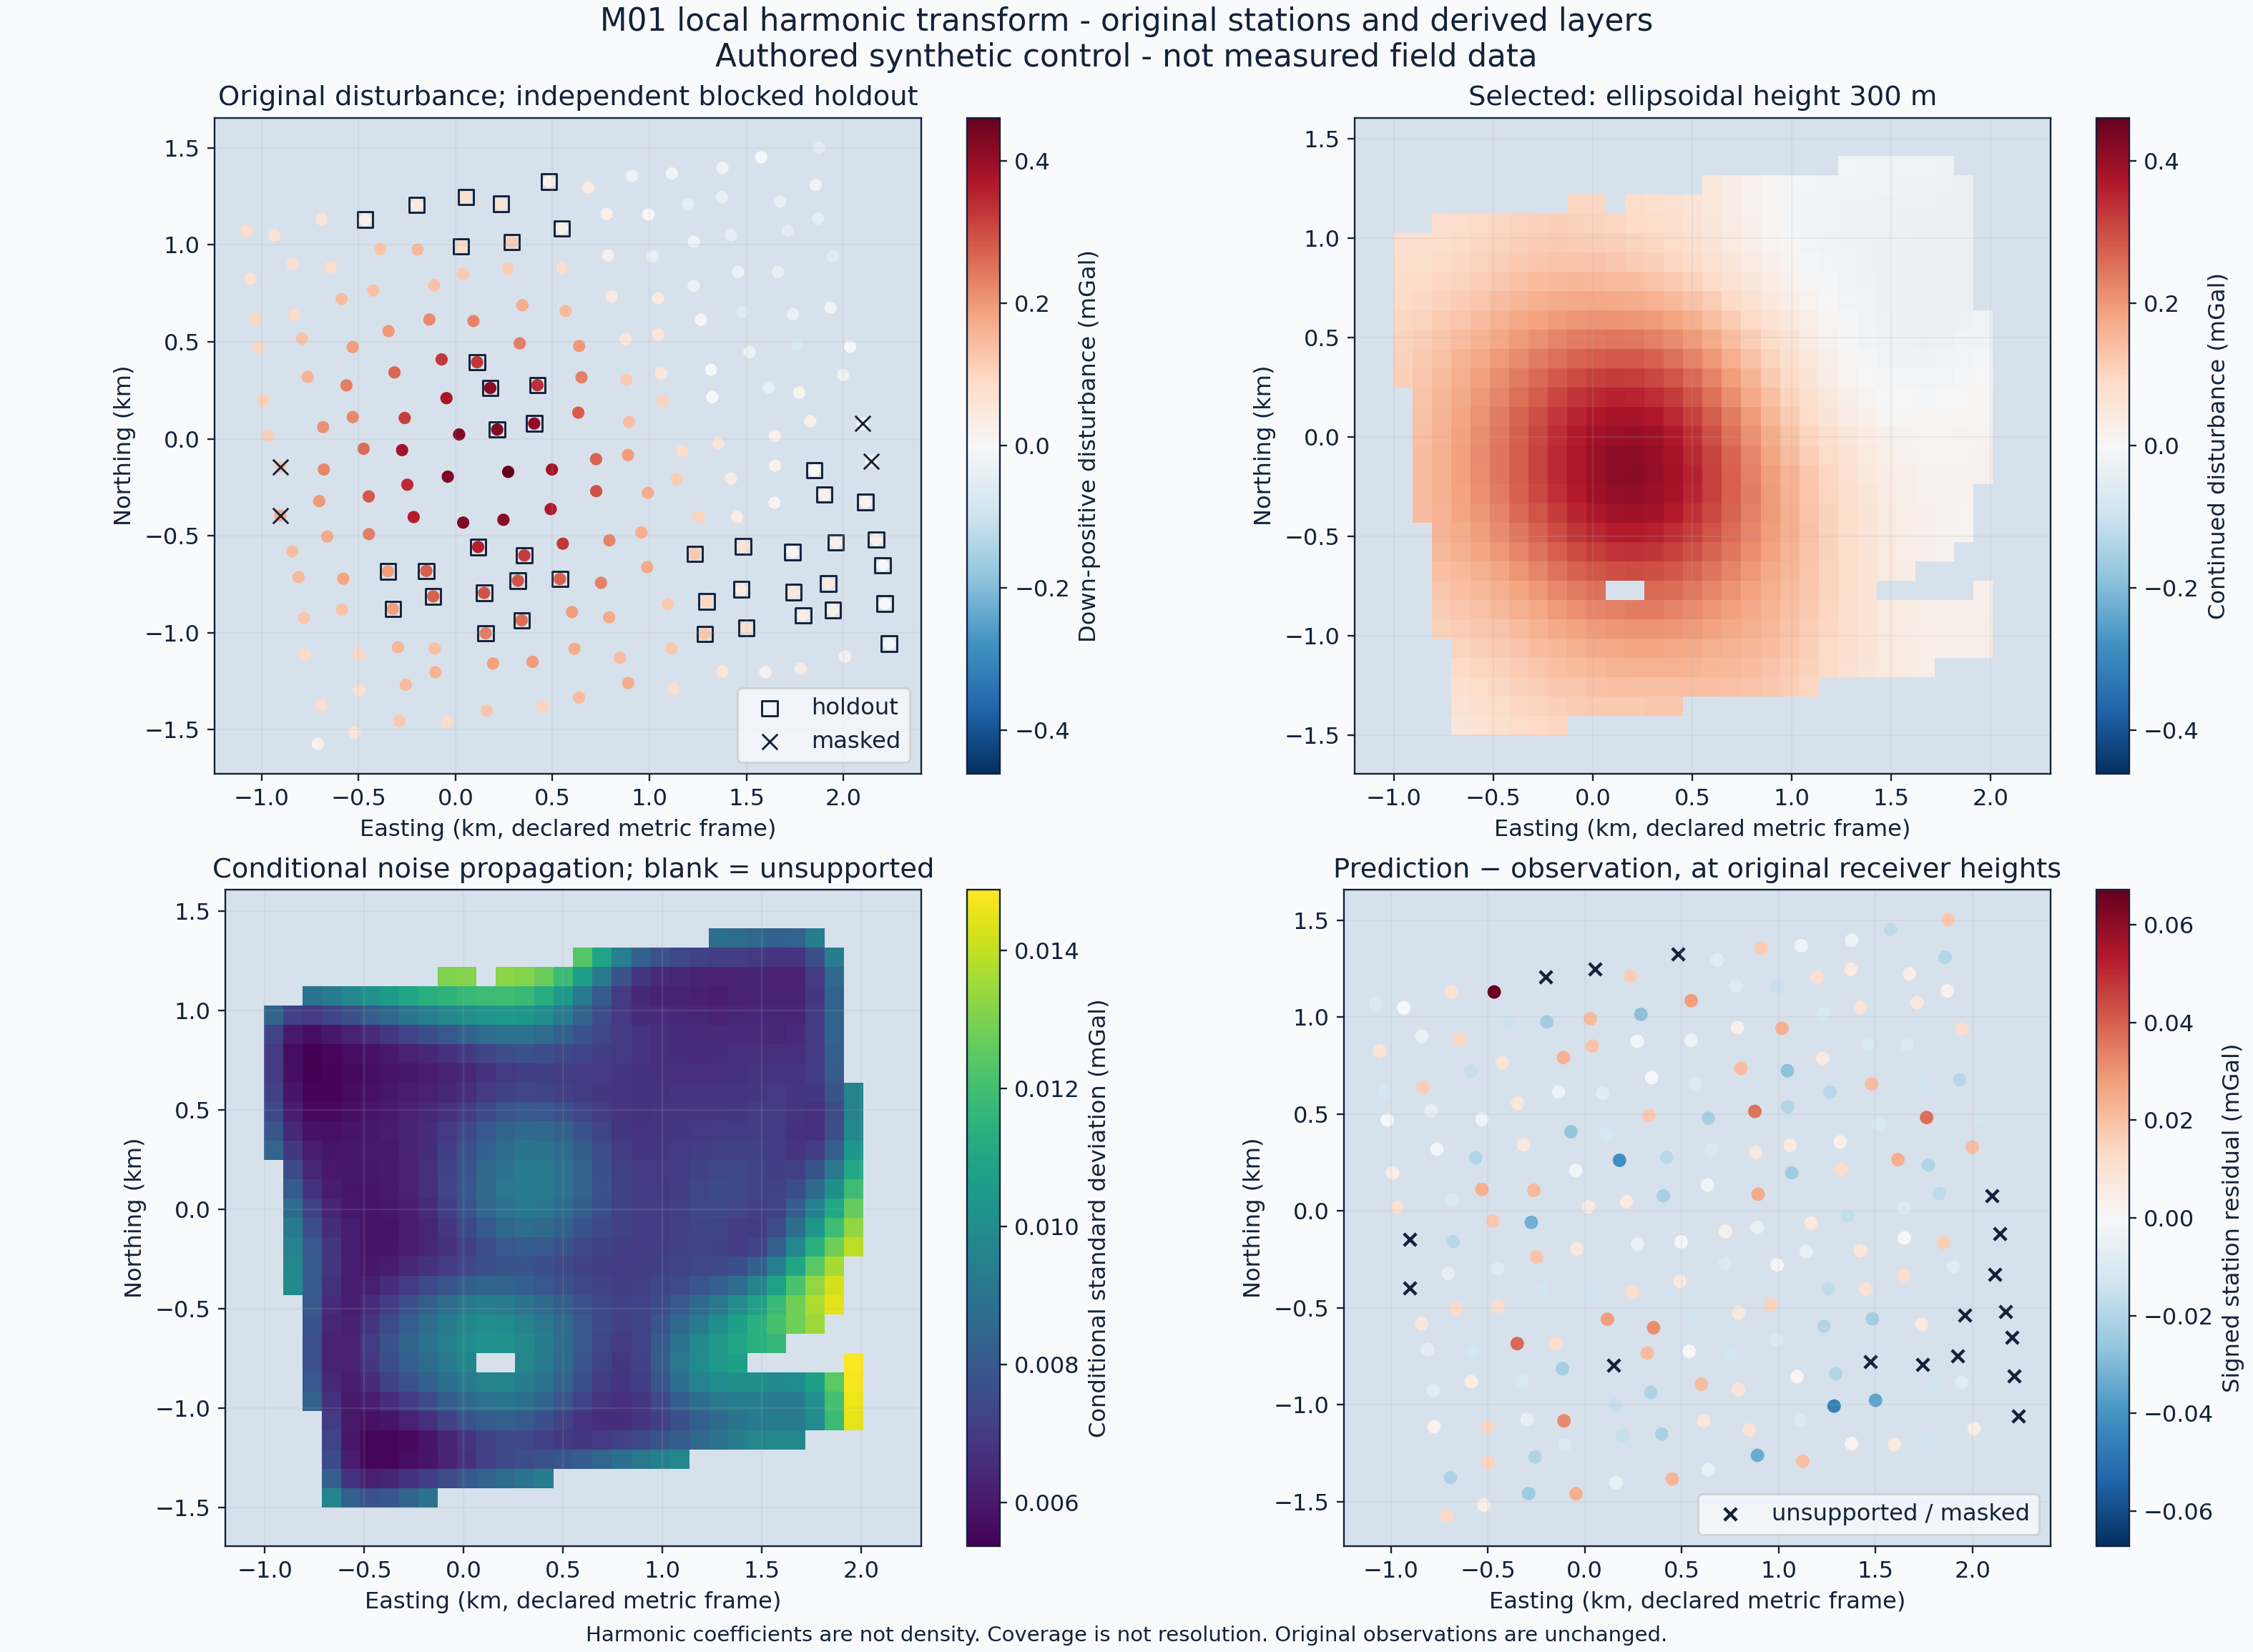
\includegraphics[width=0.95\linewidth,height=\textheight,keepaspectratio,alt={M01 authored synthetic control. Upper left: original station disturbance and blocked holdout or masked locations. Upper right: harmonic continuation to 300 m. Lower left: propagated conditional noise standard deviation, with blank cells unsupported. Lower right: signed prediction residuals at original receiver locations. The figure is synthetic and does not represent field measurements.}]{figures/m01-height-continuation.png}
\caption{M01 authored synthetic control. Upper left: original station
disturbance and blocked holdout or masked locations. Upper right:
harmonic continuation to 300 m. Lower left: propagated conditional noise
standard deviation, with blank cells unsupported. Lower right: signed
prediction residuals at original receiver locations. The figure is
synthetic and does not represent field measurements.}
\end{figure}

\subsubsection{4.2 MT, ERT, and waveform
processing}\label{mt-ert-and-waveform-processing}

The MT response is calculated through the complex impedance recursion
for isotropic layers; differentiable physics-guided inversion is a
related approach \cite{goyes2025}. EDI ingestion is a transfer-function
workflow and preserves conventions, units, rotations, masks, and stated
variances; EDI is not treated as raw time-series data. Multiple
optimizers (bounded least squares, Adam, and a small per-sounding neural
parameterization) address matched objectives in synthetic fixtures. A
neural architecture related conceptually to physics-guided inversion
\cite{goyes2025} is not asserted to reproduce the cited paper's
architecture or published results.

ERT workflows validate electrode/ABMN structure, QC and topographic
factors before inversion, following established 2D methods such as
PyGIMLi \cite{pygimli}. The numerical examples distinguish authored
controls from absent or restricted field assets and retain failed
inversions. Seismic preprocessing distinguishes instrument counts,
response-corrected units, filters, gaps, and sample windows. STA/LTA
picking and M13 learned inference consume explicitly specified traces;
analyst picks are reference annotations, not subsurface truth.

\subsubsection{4.3 Travel-time tomography, FWI, and joint
inversion}\label{travel-time-tomography-fwi-and-joint-inversion}

Travel-time inversion uses specified ray geometry and a
training/withheld partition. Its velocity maps are interpreted together
with ray support; unsupported cells do not receive equivalent evidential
status. The M09 bilingual lesson calls the product inverse core on an
authored refracting two-layer survey and compares complete withheld
shots with a training-only homogeneous baseline. This is a bounded
synthetic calculation.

The FWI implementation uses constant-density acoustic propagation
\cite{virieux2009,deepwave}, a fixed acquisition family, bounded
velocity, a data-derived coarse background, and matched update budgets
for full-band and frequency-continuation schedules. Active and withheld
receiver WRMS accompany model RMSE. A lower model RMSE can coexist with
residuals above the specified noise level. The four-case computation
includes a layered reflection, a fault, a salt/cycle-skipping negative
control, and a low-velocity channel. Its case-level results are not
generalized to field-scale FWI or elastic/attenuating physics.

Joint inversion compares uncoupled and coupled estimates against the
same observations and independent baselines. Cross-gradient coupling
promotes structural similarity, while a Gaussian-mixture prior adds a
distinct petrophysical assumption \cite{simpegJoint,astic2020}. These
mechanisms are reported separately. In the shared synthetic case,
cross-gradient slightly improves susceptibility RMSE while worsening
density RMSE relative to the optimized uncoupled solution; the
mixture-prior method slightly improves density RMSE while slightly
worsening susceptibility. Neither is a joint two-property recovery gain.
In a deliberately conflicting case, the negative control rejects a
general claim that structural or petrophysical coupling must help.

\subsubsection{4.4 Learned methods and residual
refinement}\label{learned-methods-and-residual-refinement}

The original gravity CNN predicts column density rather than a
depth-resolved volume, reflecting the non-identifiability of depth from
one potential-field map. Learned inverse benchmarks also show
sensitivity to the sampled geological families \cite{openfwi}. Its
comparison with a spatial L2 baseline uses identical seeded noisy
observations and a shared column target. The autoencoder's threshold is
selected on a separate calibration set and tested on withheld
geometries; its measured failure to detect the withheld family is
retained. These models are compact baselines and have not been compared
with a broader set of published inverse methods.

The currently submitted BS-1 paper reports a geometry-normalized,
coverage-conditioned residual CNN against a validation-selected weighted
straight-ray reference. Its input has two channels (normalized residual
and coverage); the network has 24 hidden feature maps, not 24 input
channels. The fixed protocol uses seed 77213, 40 epochs, 800 training
cases, 160 validation cases, and held-out identity, family, acquisition,
and joint shifts. On the 160-case joint holdout, the primary checkpoint
has velocity and independent travel-time RMSE ratios 2.194 and 5.585;
the second CUDA execution, with the same seed and manifests, has ratios
2.190 and 5.595. All 160 joint cases exceed each run's
validation-derived threshold. The paper therefore records a negative
result for its specified generator and operators. Repeating the same
seed measures execution sensitivity; it does not estimate
between-seed training variance. The source-bound receipts, checkpoints,
bootstrap calculation and current limitations are in
\url{manuscripts/geometry-normalized-traveltime-refinement-v001/}.

An earlier residual-v3.1/null-space experiment and its analysis remain
archived, but they are not the current BS-1 experiment. Their older
cohort, checkpoint, scorer and operator evidence cannot be combined with
the current results. The archive is retained for provenance at
\url{docs/research/archive/m12-nullspace-evaluation-draft-2026-11-13/};
the product no longer declares it as a separate proposed-method paper.
This distinction prevents the old positive aggregate ratios from being
read as results of the current method or as a beyond-state-of-the-art
claim.

\section{Selected results and
interpretation}\label{selected-results-and-interpretation}

\subsubsection{5.1 Reference-condition
outcomes}\label{reference-condition-outcomes}

The reference-condition summary lists 122 recovered, 184 unresolved, 6
failed, and 36 negative-control method results (source:
\url{docs/validation/results.md}). These are case-specific outcomes.
They must not be summed into an overall accuracy or treated as success
probabilities because the cases, units, target variables, and criteria
differ. Failure and unresolved outcomes are first-class evidence in this
project.

\subsubsection{5.2 FWI case matrix}\label{fwi-case-matrix}

The bilingual case-matrix lesson reads four hash-verified full-run
arrays (\url{notebooks/en/06-seismology/05-m10-fwi-case-matrix.ipynb};
Spanish counterpart). Layered reflection and fault are labeled recovered
under the case-specific criteria; salt remains a cycle-skipping negative
control; and the low-velocity channel remains unresolved. For the
channel, model RMSE improves relative to the starting model (ratio 0.521
for the continuation result), but fitted/withheld WRMS are 2.071/2.213
against the specified unit noise scale. This contrast shows why
improvement from a starting model is not sufficient. The notebook
re-analyzes saved output rather than re-solving FWI, and an independent
propagator comparison is needed to test sensitivity to using the same
forward engine.

\subsubsection{5.3 EDI screening and phase
picker}\label{edi-screening-and-phase-picker}

The observed cl061 EDI tensor is screened against necessary 1D
consistency conditions and fails them. It remains QC-only. It provides
no 1D resistivity model for cl061 and makes no geological interpretation
from that station. For M13, the 2026-10-27 local browser parity
computation reports all 23 valid selected display traces matching CPU
ONNX Runtime: maximum absolute probability difference 5.0664×10⁻⁶, no
P/S peak displacement, and matching accepted/abstained picks within one
sample. A twenty-fourth selected trace is QC-rejected and never
inferred. The separate locked 6,000-trace benchmark, not this curated
23-trace subset, is the population-level performance record. Even that
benchmark compares predictions with analyst annotations and should not
be described as geological truth.

\subsubsection{5.4 Novelty and null-space
assessment}\label{nullspace-novelty-assessment}

Null-space methods are established approaches for examining
non-uniqueness in travel-time tomography and seismic inversion
\cite{deWit2012,Liu2020,TorresSacchi2023}. The archived product draft
does not introduce null-space projection as new inverse theory. Its
post-hoc projection experiment also does not provide a matched current
checkpoint/operator comparison that would isolate projection as the
cause of an improvement. The archived aggregate ratios and threshold
diagnostics remain historical calculations for their stated frozen
cohorts; they are not outcomes of the current BS-1 paper and do not
establish superiority over published methods.

The current geometry-normalized residual study is likewise a bounded
synthetic comparison, not a novel solver claim. It fails both
pre-registered joint-shift error ratios for both same-seed CUDA runs.
The scientifically supported contribution is therefore a reproducible
negative comparison with explicit operators, cohort identities,
per-case diagnostics and a disclosed replay discrepancy. A new
method-performance claim would require an independent-seed training
protocol, broader generators, matched contemporary baselines, exact
operator controls and validation on eligible field observations. No
such claim is made here.

\section{Educational and visualization
design}\label{educational-and-visualization-design}

The bilingual notebook sequence covers inverse-problem foundations,
gravity, magnetics, MT, ERT, seismology, joint inversion, and learning.
Lessons include progressively deeper content: from units and forward
physics to actual solver calls, held-out evaluation, sensitivity
analyses, independent oracles, and negative controls. The notebooks are
intended as research and teaching materials, but no educational efficacy
study has been performed. The source course is cited as inspiration; its
instructional materials are not copied into the product.

Scientific visualization is organized around the method's actual state
variables. Potential-field scenes show geometry, cells, survey
observations, cuts, and physical property scales; MT views show layer
structure and frequency response; seismic instruments relate wavefields,
receiver gathers, and inversion state; learned methods show their actual
target arrays and comparison metrics. Camera rotation changes viewpoint,
not physics. Time cursors and optimizer-state replay address different
quantities and are labeled accordingly. A rendered state alone is not
evidence of uniqueness, resolution, or uncertainty.

The scientific views expose physical geometry, survey support, and
computed states. Their effect on interpretation has not been measured in
a user study, and browser performance has not been characterized across
devices, routes, languages, and themes.

\section{Computational
reproducibility}\label{computational-reproducibility}

All 60 bilingual notebooks were run from top to bottom in fresh kernels
on 30 October 2026. The computation comprised 57 unchanged notebooks and
three refreshed notebooks; none ended with an execution error. Focused
fresh-kernel replays of the refreshed examples then passed. The complete
replay used \texttt{scripts/run\_notebooks.py\ -\/-check} with external
scratch storage. Notebook sources are under \texttt{notebooks/en/} and
\texttt{notebooks/es/}.

Numerical outcomes are tied to their method-specific computation and
date. The FWI case matrix reads hash-verified outputs and does not rerun
the expensive inverse; its source is
\url{notebooks/en/06-seismology/05-m10-fwi-case-matrix.ipynb} and the
Spanish counterpart. The M12 notebook computation dated 28 October and
browser-parity computation dated 27 October are documented computations
in \url{docs/validation/m12-checkpoint-notebook-2026-10-28.md} and
\url{docs/validation/m13-browser-population-parity-2026-10-27.md}. The
null-space refinement results and cohort definitions are in
\url{docs/design/features/m12-velocity-validation/nullspace-v1_1-protocol.md}.
Reference-condition metrics are in \url{docs/validation/results.md}.
Method equations, implementation details, and primary-source mapping are
in \url{docs/research/scientific-implementation.md},
\url{docs/research/review.md}, and \url{docs/design/SDD.md}.

Notebook replay verifies execution for the recorded source and
environment; it is not an independent physical oracle. Scientific
replication requires using the method-specific data, environment, split,
seed, operator, and comparison criteria together. A lesson that reads an
archived computation must not be described as having recomputed that
solve.

\section{Limitations and open research
questions}\label{limitations-and-open-research-questions}

\begin{enumerate}
\def\labelenumi{\arabic{enumi}.}
\tightlist
\item
  \textbf{Field validation and eligibility.} Most quantitative recovery
  results are synthetic. Provider data with incomplete datum,
  uncertainty, rights, or provenance remain unresolved or ineligible.
  cl061 is a QC failure for 1D inversion, not a field inverse.
\item
  \textbf{Non-uniqueness and uncertainty.} Conditional ensembles do not
  sample geological posterior uncertainty. Potential-field structure
  remains prior- and parameterization-dependent. Coverage and
  sensitivity do not by themselves yield calibrated resolution.
\item
  \textbf{FWI scope.} The experiments use bounded acoustic physics and
  fixed synthetic acquisition families. Source uncertainty, realistic
  correlated noise, anisotropy, elasticity, attenuation, broader
  cycle-skipping regimes, and an independent propagator remain necessary
  research directions.
\item
  \textbf{Joint inversion.} Cross-gradient and mixture-prior outcomes
  depend on their scale, prior, and structural compatibility. The
  limited calibration matrix does not establish general superiority over
  optimized single-modality estimates.
\item
  \textbf{Machine learning.} The M12 learned-velocity calculation fails
  its pre-specified joint-shift comparison. The positive null-space
  variant is narrow synthetic evidence and needs external reproduction
  and broader cohorts. The phase-picker's 23-trace parity set is not an
  accuracy cohort; the separate 6,000-trace benchmark uses analyst
  annotations whose uncertainty limits the interpretation of timing
  scores.
\item
  \textbf{Data and reproducibility.} Some numerical tests require
  retained external inputs, including joint-inversion matrices and
  magnetic controls. Missing inputs are not replaced with synthetic
  stand-ins. Rights-limited source files are not copied merely to make a
  computation executable.
\item
  \textbf{Service capacity.} Local solver tests, builds, and browser
  parity do not establish worker admission, VPS capacity, cancellation,
  or recovery. Replacement-service capacity and operational behavior
  remain unmeasured.
\item
  \textbf{Educational effectiveness.} A bilingual executable notebook
  collection is a learning resource, but no controlled study establishes
  learning outcomes or comparative pedagogical effectiveness.
\end{enumerate}

Useful next studies include preregistered geological-family and
acquisition/noise ensembles; matched contemporary travel-time baselines;
independent-seed training and calibration under forward-model and
geological uncertainty; independent FWI propagation; licensed field
inversions with source/datum/error review; and user studies of whether
linking assumptions, predictions, residuals, and uncertainty improves
interpretation.

\section{Conclusions}\label{conclusions}

Inverse Earth Studio combines source-linked geophysical processing and
inverse methods with explicit assumptions, independent physical checks
where available, and preserved negative evidence. Its central examples
show that data fit, model recovery, transfer, and visual plausibility
are different questions. The workbench includes synthetic and bounded
real-data screening calculations, bilingual executable notebooks, and
computational paths across multiple physical methods.

These computations do not establish field validity or generality across
geological settings. Several method-specific comparisons, end-to-end
user-supplied-data workflows, actual-host measurements, independent
solver comparisons, and user-facing visual evaluations remain to be
completed. The current learned travel-time refinement fails its two
joint-shift error criteria in the primary run and a same-seed replay.
The earlier null-space draft is archived as a historical analysis of an
established operation, not as a novel method. The work provides a
reproducible software and experimental framework that makes assumptions
and counterexamples inspectable. Algorithmic novelty and publication
priority are not established.

\section{Data and code availability}\label{data-and-code-availability}

Source code is available at
\texttt{https://github.com/fsantibanezleal/CAOS\_Geophysics}. Scientific
methods, notebooks, test data, computational records, and source-rights
decisions are linked above and organized in \texttt{data/},
\texttt{data-pipeline/}, \texttt{docs/}, \texttt{notebooks/},
\texttt{tests/}, and \texttt{models/}. Some external raw observations
are absent because redistribution rights or field eligibility remain
unresolved. The intended application origin is
\texttt{https://geophysics.ml.fasl-work.com/}. Local computations do not
establish replacement-service capacity.

\section{Acknowledgements}\label{acknowledgements}

The work uses and cites open scientific software and public geophysical
data sources listed below and in the repository's research review. No
endorsement by the cited software or dataset authors is implied.
